%% main.tex <- USPSC-TCC-modelo.tex
% ---------------------------------------------------------------
% USPSC: Modelo de Trabalho Academico (tese de doutorado, dissertacao de
% mestrado e trabalhos monograficos em geral) em conformidade com 
% ABNT NBR 14724:2011: Informacao e documentacao - Trabalhos academicos -
% Apresentacao
%----------------------------------------------------------------
%% Esta é uma customização do abntex2-modelo-trabalho-academico.tex de v-1.9.5 laurocesar 
%% para as Unidades do Campus USP de São Carlos:
%% EESC - Escola de Engenharia de São Carlos
%% IAU - Instituto de Arquitetura e Urbanismo
%% ICMC - Instituto de Ciências Matemáticas e de Computação
%% IFSC - Instituto de Física de São Carlos
%% IQSC - Instituto de Química de São Carlos
%%
%% Este trabalho utiliza a classe USPSC.cls que é mantida pela seguinte equipe:
%% 
%% Coordenação e Programação:
%%   - Marilza Aparecida Rodrigues Tognetti - marilza@sc.usp.br (PUSP-SC)
%%   - Ana Paula Aparecida Calabrez - aninha@sc.usp.br (PUSP-SC)
%% Normalização:
%%   - Brianda de Oliveira Ordonho Sigolo - brianda@usp.br (IAU)
%%   - Eduardo Graziosi Silva - edu.gs@sc.usp.br (EESC)
%%   - Eliana de Cássia Aquareli Cordeiro - eliana@iqsc.usp.br (IQSC)
%%   - Flávia Helena Cassin - cassinp@sc.usp.br (EESC)
%%   - Maria Cristina Cavarette Dziabas - mcdziaba@ifsc.usp.br (IFSC)
%%   - Regina Célia Vidal Medeiros - rcvmat@icmc.usp.br (ICMC)
%%
%% O USPSC-modelo.tex e USPSC-TCC-modelo.tex utilizam diversos arquivos relacionado em 
%% 2.1 Pacote USPSC: Classe USPSC e modelos de trabalhos acadêmicos	do Tutorial do Pascote 
%%  USPSC para modelos de trabalhos de acadêmicos em LaTeX - versão 3.1


%----------------------------------------------------------------
%% Sobre a classe abntex2.cls:
%% abntex2.cls, v-1.9.5 laurocesar
%% Copyright 2012-2015 by abnTeX2 group at https://www.abntex.net.br/ 
%%
%----------------------------------------------------------------

\documentclass[
% -- opções da classe memoir --
12pt,		% tamanho da fonte
openright,	% capítulos começam em pág ímpar (insere página vazia caso preciso)
%twoside,  % para impressão em anverso (frente) e verso. Oposto a oneside
oneside, % para impressão em páginas separadas (somente anverso)
a4paper,			% tamanho do papel. 
% -- opções da classe abntex2 --
chapter=TITLE,		% títulos de capítulos convertidos em letras maiúsculas
% -- opções do pacote babel --
english,			% idioma adicional para hifenização
french,				% idioma adicional para hifenização
spanish,			% idioma adicional para hifenização
brazil				% o último idioma é o principal do documento
% {USPSC-classe/USPSC} configura o cabeçalho contendo apenas o número da página
]{USPSC-classe/USPSC}
%]{USPSC-classe/USPSC1}
% Inclua % antes de ]{USPSC-classe/USPSC} e retire a % antes de %]{USPSC-classe/USPSC1} para utilizar o 
% cabeçalho diferenciado para as páginas pares e ímpares:
%- páginas ímpares: com seções ou subseções e o número da página
%- páginas pares: com o número da página e o título do capítulo 
% ---
% ---
% Pacotes básicos - Fundamentais 
% ---
\usepackage[T1]{fontenc}		% Seleção de códigos de fonte.
\usepackage[utf8]{inputenc}		% Codificação do documento (conversão automática dos acentos)
\usepackage{lmodern}			% Usa a fonte Latin Modern
% Para utilizar a fonte Times New Roman, inclua uma % no início do comando acima  "\usepackage{lmodern}"
% Abaixo, tire a % antes do comando  \usepackage{times}
%\usepackage{times}		    	% Usa a fonte Times New Roman	
% Para usar a fonte , lembre-se de tirar a % do comando %\renewcommand{\ABNTEXchapterfont}{\rmfamily}, localizado mais abaixo, logo após "Outras opções para nota de rodapé no Sistema Numérico" 					
\usepackage{lastpage}			% Usado pela Ficha catalográfica
\usepackage{indentfirst}		% Indenta o primeiro parágrafo de cada seção.
\usepackage{color}				% Controle das cores
\usepackage{graphicx}			% Inclusão de gráficos
\usepackage{float} 				% Fixa tabelas e figuras no local exato
\usepackage{lipsum}  
\usepackage{tikz}				% Para escrever reações químicas e outros
%\usetikzlibrary{positioning}
\usetikzlibrary{shapes,positioning,calc,quotes}
\tikzstyle{subrotina} = [rectangle, draw,text centered, minimum width=5em, inner sep=5pt]

\tikzstyle{funcao} = [rounded rectangle, draw, text centered, minimum width=7em, inner sep=5pt]

\tikzstyle{random} = [rectangle, text centered, inner sep=5pt, minimum width=5em]

\tikzstyle{loop} = [rectangle, draw, align=left]

\tikzstyle{fluxo} = [draw, thick, -latex]

\tikzstyle{meiofluxo} = [draw, -]

\tikzstyle{chamada} = [draw, dashed, <->]
%\tikzset{
%	basic box/.style={
%		shape=rectangle, rounded corners, align=center, draw=#1, fill=#1!25},
%	header node/.style={
%		node family/width=header nodes,
%		font=\strut\Large\ttfamily,
%		text depth=+.3ex, fill=white, draw},
%	header/.style={%
%		inner ysep=+1.5em,
%		append after command={
%			\pgfextra{\let\TikZlastnode\tikzlastnode}
%			node [header node] (header-\TikZlastnode) at (\TikZlastnode.north) {#1}
%			% the next node contains both \tikzlastnode and its header
%			% this is needed so that h- can be used to connect lines
%			node [span=(\TikZlastnode)(header-\TikZlastnode)]
%			at (fit bounding box) (h-\TikZlastnode) {}
%		}
%	},
%	fat blue line/.style={ultra thick, blue}
%}
\usepackage{microtype} 			% para melhorias de justificação
\usepackage{pdfpages}
\usepackage{makeidx}            % para gerar índice remissivo
\usepackage{hyphenat}          % Pacote para retirar a hifenizacao do texto
\usepackage[absolute]{textpos} % Pacote permite o posicionamento do texto
\usepackage{eso-pic}           % Pacote para incluir imagem de fundo
\usepackage{makebox}  
\usepackage{amsmath}
\usepackage[superscript]{cite} % agrupa citações numéricas consecutivas
\usepackage[num, abnt-emphasize=bf, abnt-thesis-year=both, abnt-repeated-author-omit=no, abnt-last-names=abnt, abnt-etal-cite, abnt-etal-list=3, abnt-etal-text=it, abnt-and-type=e, abnt-doi=doi, abnt-url-package=none, abnt-verbatim-entry=no]{abntex2cite} 
\bibliographystyle{USPSC-classe/abntex2-num-USPSC}

\renewcommand{\thefootnote}{\fnsymbol{footnote}}  %Comando para inserção de símbolos em nota de rodapé

\renewcommand{\footnotesize}{\small} %Comando para diminuir a fonte das notas de rodapé

% ---
% Pacotes adicionais, usados apenas no âmbito do Modelo Canônico do abnteX2
% ---
\usepackage{lipsum}				% para geração de dummy text
% ---

% pacotes de tabelas
\usepackage{multicol}	% Suporte a mesclagens em colunas
\usepackage{multirow}	% Suporte a mesclagens em linhas
\usepackage{longtable}	% Tabelas com várias páginas
\usepackage{threeparttablex}    % notas no longtable
\usepackage{array}

\usepackage{physics}
\usepackage{bbold}
\usepackage{subcaption}

% ----
% Compatibilização com a ABNT NBR 6023:2018
% Para tirar <> da URL
%\DeclareFieldFormat{url}{\bibstring{urlfrom}\addcolon\addspace\url{#1}}
\usepackage{USPSC-classe/ABNT6023-2018}
% As demais compatibilizações estão nos arquivos abntex2-alf-USPSC.bst,abntex2-alfeng-USPSC.bst, abntex2-num-USPSC.bst e abntex2-numeng-USPSC.bst, dependendo do idioma do textos e se o sistemas de chamada for autor-data ou numérico, conforme explicitado acima.
% ----

% ---
% DADOS INICIAIS - Define sigla com título, área de concentração e opção do Programa 
\siglaunidade{IFSC-TCC}
\programa{BFCp}

% Configurações de aparência do PDF final
% alterando o aspecto da cor azul
\definecolor{blue}{RGB}{41,5,195}


% informações do PDF
\makeatletter
\hypersetup{
	%pagebackref=true,
	pdftitle={\@title}, 
	pdfauthor={\@author},
	pdfsubject={\imprimirpreambulo},
	pdfcreator={LaTeX with abnTeX2},
	pdfkeywords={abnt}{latex}{abntex}{USPSC}{trabalho acadêmico}, 
	colorlinks=true,       		% false: boxed links; true: colored links
	linkcolor=black,          	% color of internal links
	citecolor=black,        		% color of links to bibliography
	filecolor=black,      		% color of file links
	urlcolor=black,
	%Para habilitar as cores dos links, retire a % antes dos comandos abaixo e inclua a % antes das 4 linhas de comando acima 
	%linkcolor=blue,            	% color of internal links
	%citecolor=blue,        		% color of links to bibliography
	%filecolor=magenta,      		% color of file links
	%urlcolor=blue,
	bookmarksdepth=4	
}
\makeatother
% --- 
% --- 
% Espaçamentos entre linhas e parágrafos 
% --- 

% O tamanho do parágrafo é dado por:
\setlength{\parindent}{1.3cm}

% Controle do espaçamento entre um parágrafo e outro:
\setlength{\parskip}{0.2cm}  % tente também \onelineskip

% ---
% compila o sumário e índice
\makeindex
% ---

% ----------------

\newcommand\underrel[2]{\mathrel{\mathop{#2}\limits_{#1}}}

\newcommand{\matriz}[1]{\hat#1}

\newcommand{\many}[2]{$#1_1, #1_2, \dots, #1_#2$}

\newcommand{\cmany}[3]{$#1_1 #3 #1_2 #3 \dots #3 #1_#2$}

\newcommand{\mmany}[2]{ #1_1, #1_2, \dots, #1_#2 }

\newcommand{\mcmany}[3]{#1_1 #3 #1_2 #3 \dots #3 #1_#2}

\newcommand{\set}[1]{\{#1\}}

\newcommand{\cjgt}[1]{\overline{#1}}
\DeclareMathOperator{\diag}{diag}
\DeclareMathOperator{\sign}{sign}
\DeclareMathOperator{\ai}{Ai}
\DeclareMathOperator{\re}{Re}
\DeclareMathOperator{\im}{Im}
\DeclareMathOperator{\Df}{D}
\DeclareMathOperator{\Ee}{E}
\DeclareMathOperator{\h}{h_1}
\DeclareMathOperator{\f}{f}
\DeclareMathOperator{\U}{U}
\DeclareMathOperator{\W}{W}
\DeclareMathOperator{\K}{K}
\DeclareMathOperator{\Hf}{\mathcal{H}}
\DeclareMathOperator{\Qf}{Q}
\DeclareMathOperator{\Gl}{\mathcal{L}}
\DeclareMathOperator{\g}{g}
\DeclareMathOperator{\V}{V}
\newcommand{\iu}{\mathrm{i}\mkern1mu}
\renewcommand{\Im}{\mathop{\textrm Im}}
\DeclareMathOperator{\ee}{e}
\DeclareMathOperator{\supp}{supp}
\newcommand{\N}{\mathbb{N}}
\newcommand{\C}{\mathbb{C}}
\newcommand{\R}{\mathbb{R}}
\newcommand{\Z}{\mathbb{Z}}
\newcommand{\D}{\mathbb{D}}
\newcommand{\Q}{\mathbb{Q}}
\newcommand{\J}{J} %Jacobiano
\newcommand{\Id}{\mathbb{1}}
\newcommand{\p}{p} %medida
\newcommand{\E}{\mathbb{E}}
\newcommand{\Se}{\mathbb{S}}
\newcommand{\He}{\mathbb{H}}
\newcommand{\boh}{\mathit{o}}
\newcommand{\Boh}{\mathcal{O}}
\newcommand{\bbp}{\bm K_{\mathrm{BBP}}}
\newcommand{\ii}{\mathrm{i}}
\newcommand*{\deff}{\mathrel{\vcenter{\baselineskip0.5ex \lineskiplimit0pt
			\hbox{\scriptsize.}\hbox{\scriptsize.}}}%
	=}
\newcommand*{\revdeff}{=\mathrel{\vcenter{\baselineskip0.5ex \lineskiplimit0pt
			\hbox{\scriptsize.}\hbox{\scriptsize.}}}%
}


% MATH DECLARATIONS
\newtheorem{lemma}{Lema}[section]
\newtheorem{thm}[lemma]{Teorema}
\newtheorem{claim}[lemma]{Afirmação}
\newtheorem{cor}[lemma]{Corolário}
\newtheorem{definition}[lemma]{Definição}
\newtheorem{conjecture}[lemma]{Conjectura}
\newtheorem{prop}[lemma]{Proposição}
\newtheorem{assumption}[lemma]{Assumpção}
\numberwithin{equation}{section} %numeracao dentro de secoes

% PROOF ENV
\makeatletter
\newenvironment{proof}[1][Demonstração]{\par
	\pushQED{\qed}%
	\normalfont \topsep6\p@\@plus6\p@\relax
	\trivlist
	\item\relax
	{\itshape
		#1\@addpunct{.}}\hspace\labelsep\ignorespaces
}{%
	\popQED\endtrivlist\@endpefalse
}
\makeatother

%-----------

% ----
% Início do documento
% ----
\begin{document}

% Seleciona o idioma do documento (conforme pacotes do babel)
\selectlanguage{brazil}
% Se o idioma do texto for inglês, inclua uma % antes do 
%      comando \selectlanguage{brazil} e 
%      retire a % antes do comando abaixo
%\selectlanguage{english}

% Retira espaço extra obsoleto entre as frases.
\frenchspacing 

% --- Formatação dos Títulos
\renewcommand{\ABNTEXchapterfontsize}{\fontsize{12}{12}\bfseries}
\renewcommand{\ABNTEXsectionfontsize}{\fontsize{12}{12}\bfseries}
\renewcommand{\ABNTEXsubsectionfontsize}{\fontsize{12}{12}\normalfont}
\renewcommand{\ABNTEXsubsubsectionfontsize}{\fontsize{12}{12}\normalfont}
\renewcommand{\ABNTEXsubsubsubsectionfontsize}{\fontsize{12}{12}\normalfont}


% ----------------------------------------------------------
% ELEMENTOS PRÉ-TEXTUAIS
% ----------------------------------------------------------
% ---
% Capa
% ---
\imprimircapa
% ---
% Folha de rosto
% (o * indica impressão em anverso (frente) e verso )
% ---
\imprimirfolhaderosto*
%\imprimirfolhaderosto
% ---
% ---
% Inserir a ficha catalográfica em pdf
% ---
% A biblioteca da sua Unidade lhe fornecerá um PDF com a ficha
% catalográfica definitiva. 
% Quando estiver com o documento, salve-o como PDF no diretório
% do seu projeto como fichacatalografica.pdf e inclua o arquivo
% utilizando o comando abaixo:

%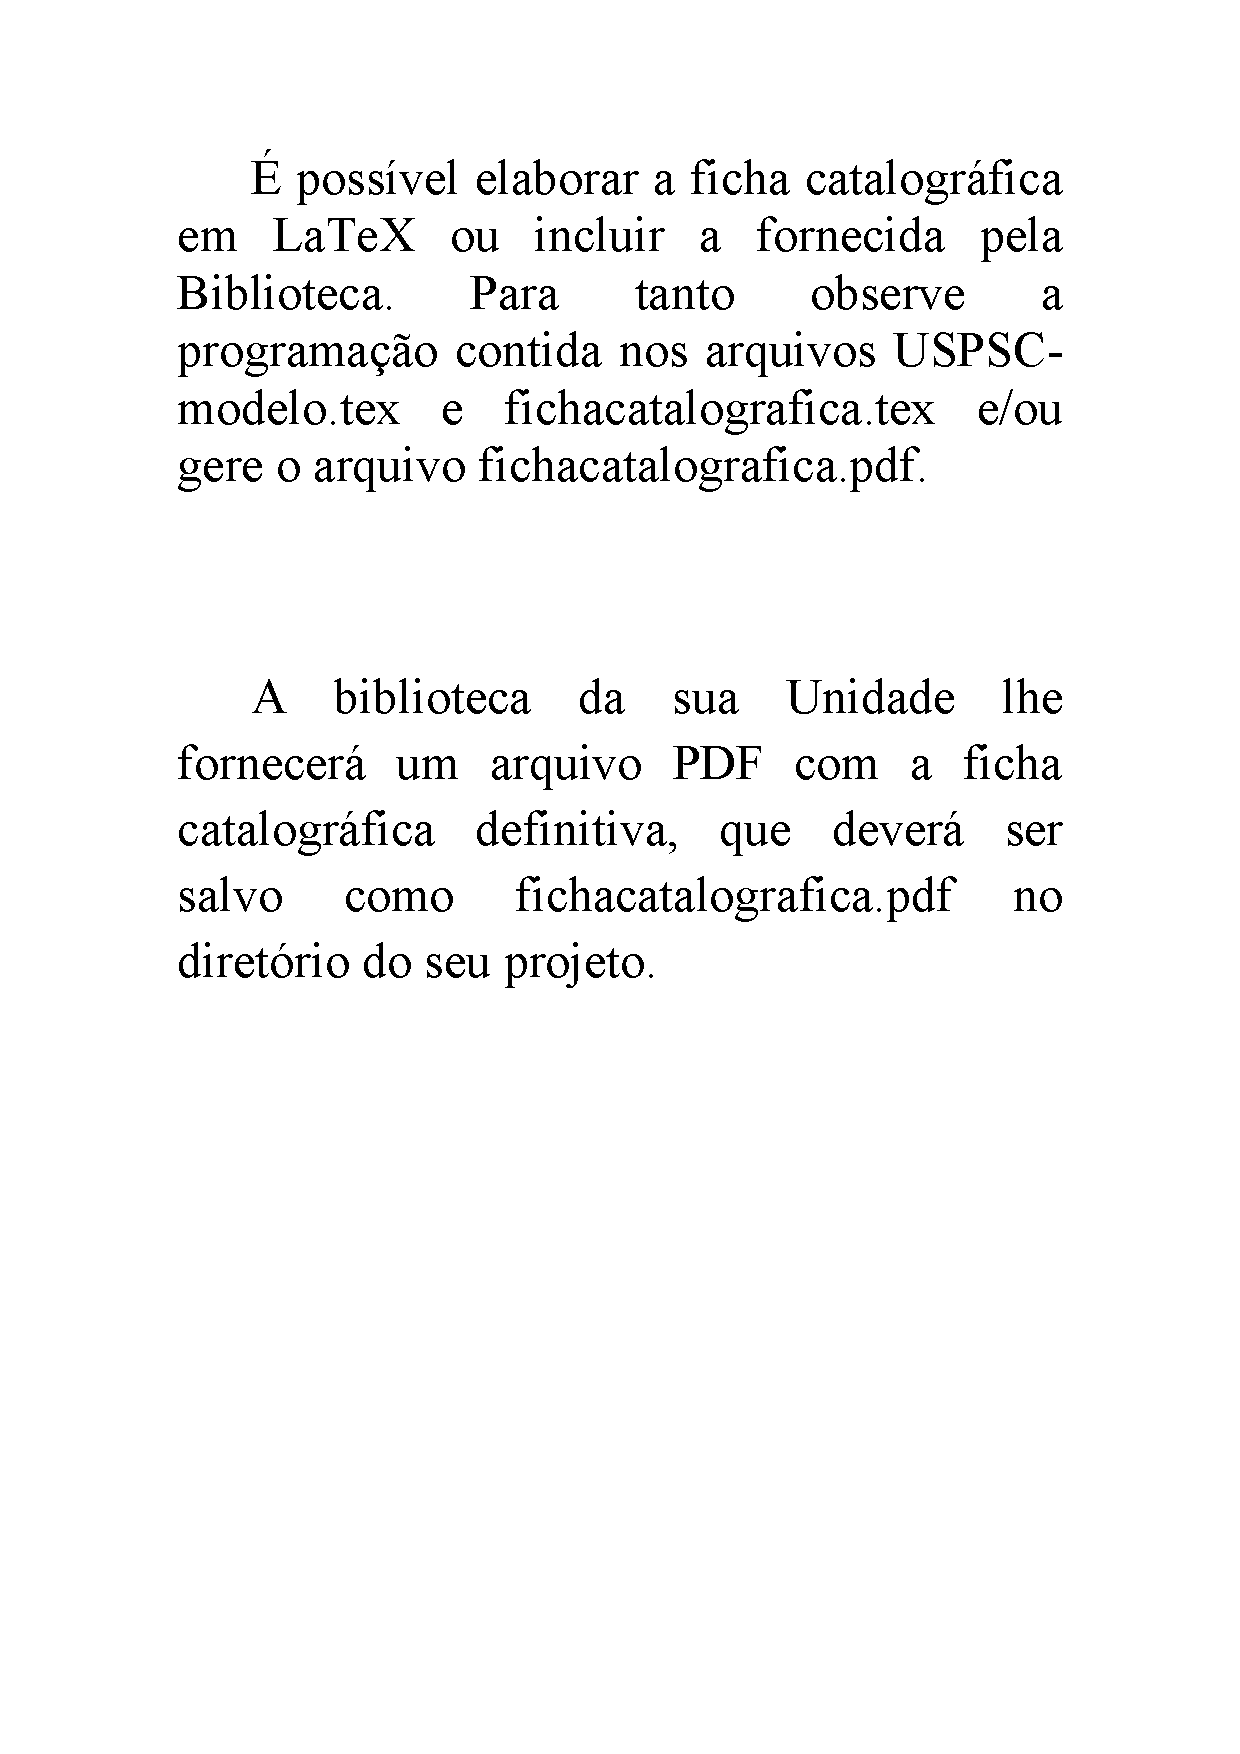
\includepdf{USPSC-TA-PreTextual/USPSC-fichacatalografica.pdf}

% Se você optar por elaborar a ficha catalográfica, deverá 
% incluir uma % antes da linha % antes
% do comando %% USPSC-fichacatalografica.tex
% ---
% Inserir a ficha bibliografica
% ---
% Isto é um exemplo de Ficha Catalográfica, ou ``Dados internacionais de
% catalogação-na-publicação''. Você pode utilizar este modelo como referência. 
% Porém, provavelmente a biblioteca da sua universidade lhe fornecerá um PDF
% com a ficha catalográfica definitiva após a defesa do trabalho. Quando estiver
% com o documento, salve-o como PDF no diretório do seu projeto e substitua todo
% o conteúdo de implementação deste arquivo pelo comando abaixo:
%
\begin{fichacatalografica}
	\hspace{-1.4cm}
	\imprimirnotaautorizacao \\ \\
	%\sffamily
	\vspace*{\fill}					% Posição vertical
\begin{center}					% Minipage Centralizado
  \imprimirnotabib \\
  \begin{table}[htb]
	\scriptsize
	\centering	
	\begin{tabular}{|p{0.9cm} p{8.7cm}|}
		\hline
	      & \\
		  &	  \imprimirautorficha     \\
		
		 \imprimircutter & 
							\hspace{0.4cm}\imprimirtitulo~  / ~\imprimirautor~ ;  ~\imprimirorientadorcorpoficha. -- 	\imprimirlocal, \imprimirdata.   \\
		
		  &  % Para incluir nota referente à versão corrigida no corpo da ficha,
			  % incluir % no início da linha acima e tirar a % do início da linha abaixo
			  %	\hspace{0.4cm} \imprimirtitulo~  / ~\imprimirautor~ ; ~\imprimirorientadorcorpoficha~- ~\imprimirnotafolharosto. -- \imprimirlocal, \imprimirdata.  \\
		
			\hspace{0.4cm}\pageref{LastPage} p.\\ 
		  & \\
		  & 
		    \hspace{0.4cm}\imprimirnotaficha ~--~ 
						  \imprimirunidademin, 
						  \imprimiruniversidademin, 
		                  \imprimirdata. \\ 
		  & \\                 
		   % Para incluir nota referente à versão corrigida em notas,
		    % incluir uma % no início da linha acima e	
		    % tirar a % do início da linha abaixo
		    % & \hspace{0.4cm}\imprimirnotafolharosto \\ 
		  & \\ 
		  & \hspace{0.4cm}1. Introdução. 2. Matrizes Aleatórias. 3. Simulações e Algoritmos. 4. Implementação e Resultados 5. Conclusão. I. \imprimirorientadorficha. II. Matrizes Aleatórias e Simulação de Gases de Coulomb. \\
	
		     %Se houver co-orientador, inclua % antes da linha (antes de II. Título.) 
		     %          e tire a % antes do comando abaixo 
		     %III. Título. \\   
		  \hline
	\end{tabular}
  \end{table}
\end{center}
\end{fichacatalografica}
% ---

 
% e retirar o % do comando abaixo
%% USPSC-fichacatalografica.tex
% ---
% Inserir a ficha bibliografica
% ---
% Isto é um exemplo de Ficha Catalográfica, ou ``Dados internacionais de
% catalogação-na-publicação''. Você pode utilizar este modelo como referência. 
% Porém, provavelmente a biblioteca da sua universidade lhe fornecerá um PDF
% com a ficha catalográfica definitiva após a defesa do trabalho. Quando estiver
% com o documento, salve-o como PDF no diretório do seu projeto e substitua todo
% o conteúdo de implementação deste arquivo pelo comando abaixo:
%
\begin{fichacatalografica}
	\hspace{-1.4cm}
	\imprimirnotaautorizacao \\ \\
	%\sffamily
	\vspace*{\fill}					% Posição vertical
\begin{center}					% Minipage Centralizado
  \imprimirnotabib \\
  \begin{table}[htb]
	\scriptsize
	\centering	
	\begin{tabular}{|p{0.9cm} p{8.7cm}|}
		\hline
	      & \\
		  &	  \imprimirautorficha     \\
		
		 \imprimircutter & 
							\hspace{0.4cm}\imprimirtitulo~  / ~\imprimirautor~ ;  ~\imprimirorientadorcorpoficha. -- 	\imprimirlocal, \imprimirdata.   \\
		
		  &  % Para incluir nota referente à versão corrigida no corpo da ficha,
			  % incluir % no início da linha acima e tirar a % do início da linha abaixo
			  %	\hspace{0.4cm} \imprimirtitulo~  / ~\imprimirautor~ ; ~\imprimirorientadorcorpoficha~- ~\imprimirnotafolharosto. -- \imprimirlocal, \imprimirdata.  \\
		
			\hspace{0.4cm}\pageref{LastPage} p.\\ 
		  & \\
		  & 
		    \hspace{0.4cm}\imprimirnotaficha ~--~ 
						  \imprimirunidademin, 
						  \imprimiruniversidademin, 
		                  \imprimirdata. \\ 
		  & \\                 
		   % Para incluir nota referente à versão corrigida em notas,
		    % incluir uma % no início da linha acima e	
		    % tirar a % do início da linha abaixo
		    % & \hspace{0.4cm}\imprimirnotafolharosto \\ 
		  & \\ 
		  & \hspace{0.4cm}1. Introdução. 2. Matrizes Aleatórias. 3. Simulações e Algoritmos. 4. Implementação e Resultados 5. Conclusão. I. \imprimirorientadorficha. II. Matrizes Aleatórias e Simulação de Gases de Coulomb. \\
	
		     %Se houver co-orientador, inclua % antes da linha (antes de II. Título.) 
		     %          e tire a % antes do comando abaixo 
		     %III. Título. \\   
		  \hline
	\end{tabular}
  \end{table}
\end{center}
\end{fichacatalografica}
% ---


% As informações que compõem a ficha catalográfica estão 
% definidas no arquivo USPSC-pre-textual-UUUU.tex
% ---

% ---
% ---
% Inserir errata
% ---

%%% USPSC-Errata.tex
\begin{errata}
	%\OnehalfSpacing 			
	A errata é um elemento opcional, que consiste de uma lista de erros da obra, precedidos pelas folhas e linhas onde eles ocorrem e seguidos pelas correções correspondentes. Deve ser inserida logo após a folha de rosto e conter a referência do trabalho para facilitar sua identificação, conforme a ABNT NBR 14724 \cite{nbr14724}.
	
	Modelo de Errata:
		
	\begin{flushleft} 
			\setlength{\absparsep}{0pt} % ajusta o espaçamento da referência	
			\SingleSpacing 
			\imprimirautorabr~ ~\textbf{\imprimirtituloresumo}.	\imprimirdata. \pageref{LastPage}p. 
			%Substitua p. por f. quando utilizar oneside em \documentclass
			%\pageref{LastPage}f.
			\imprimirtipotrabalho~-~\imprimirinstituicao, \imprimirlocal, \imprimirdata. 
 	\end{flushleft}
\vspace{\onelineskip}
\OnehalfSpacing 
\center
\textbf{ERRATA}
\vspace{\onelineskip}
\OnehalfSpacing 
\begin{table}[htb]
	\center
	\footnotesize
	\begin{tabular}{p{2cm} p{2cm} p{4cm} p{4cm} }
		\hline
		\textbf{Folha} & \textbf{Linha}  & \textbf{Onde se lê}  & \textbf{Leia-se}  \\
			\hline
			1 & 10 & auto-conclavo & autoconclavo\\
		\hline
	\end{tabular}
\end{table}
\end{errata}
% ---

% ---

% ---
% Inserir folha de aprovação
% ---

% A Folha de aprovação é um elemento obrigatório da NBR 4724/2011 (seção 4.2.1.3). 
% Após a defesa/aprovação do trabalho, gere o arquivo folhadeaprovacao.pdf da página assinada pela banca 
% e iclua o arquivo utilizando o comando abaixo:
%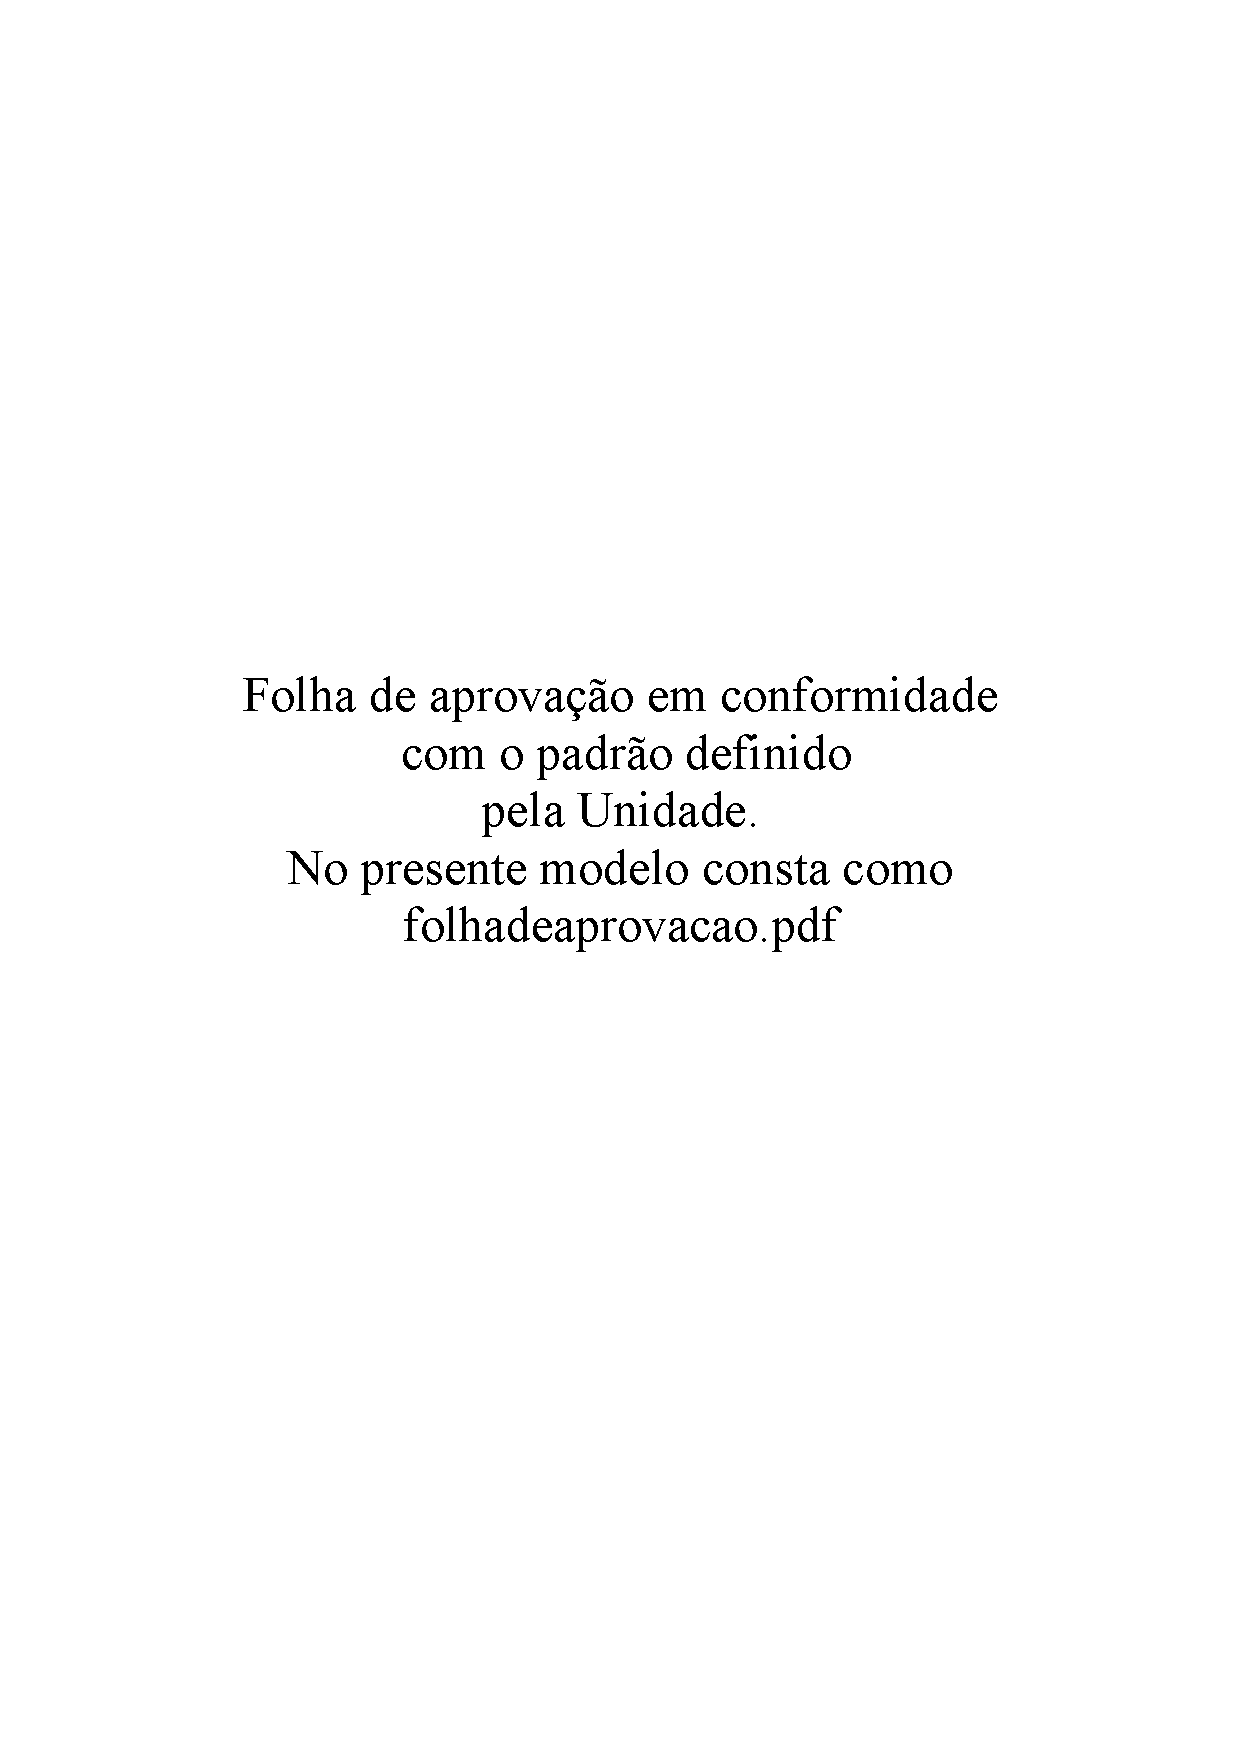
\includepdf{USPSC-TA-PreTextual/USPSC-folhadeaprovacao.pdf}
% Alternativa para a Folha de Aprovação:
% Se for a sua opção elaborar uma folha de aprovação, insira uma % antes do comando acima que inclui o arquivo folhadeaprovacao.pdf,
% tire o % do comando abaixo e altere o arquivo folhadeaprovacao.tex conforme suas necessidades
%\include{folhadeaprovacao}
%
\includepdf{USPSC-TA-PreTextual/USPSC-PaginaEmBranco.pdf}

% ---
% Dedicatória
% ---
%%% USPSC-Dedicatoria.tex
\begin{dedicatoria}
   \vspace*{\fill}
   \centering
   \noindent
   \textit{ Este trabalho é dedicado aos alunos da USP, como uma contribuição\\
  das Bibliotecas do Campus USP de São Carlos para o desenvolvimento\\
	e disseminação da pesquisa científica da Universidade.} \vspace*{\fill}
\end{dedicatoria}
% ---
% ---

% ---
% Agradecimentos
% ---
%%% USPSC-Agradecimentos.tex
\begin{agradecimentos}
	Primeira frase do agradecimento ....
	
	Segunda frase ....
	
	Outras frases ....
	
	Última frase ....
	
\end{agradecimentos}
% ---
% ---

% ---
% Epígrafe
% ---
%%% USPSC-Epigrafe.tex
\begin{epigrafe}
    \vspace*{\fill}
	\begin{flushright}
		\textit{"En remontant chez moi pour y passer la soirée à travailler de mon mieux, je me disais que le monde n'est pas construit pour l'équilibre. Le monde est désordre. L'équilibre n'est pas la règle, c'est l'exception."\\
		G.Duhamel, Maitres, 1937}
	\end{flushright}
\end{epigrafe}
% ---
% ---

% A T E N Ç Ã O
% Se o idioma do texto for em inglês, o abstract deve preceder o resumo
% resumo em português
%
% Resumo
% ---
%% USPSC-Resumo.tex
\setlength{\absparsep}{18pt} % ajusta o espaçamento dos parágrafos do resumo		
\begin{resumo}
	\begin{flushleft} 
			\setlength{\absparsep}{0pt} % ajusta o espaçamento da referência	
			\SingleSpacing 
			\imprimirautorabr~~\textbf{\imprimirtituloresumo}.	\imprimirdata. \pageref{LastPage}p. 
			%Substitua p. por f. quando utilizar oneside em \documentclass
			%\pageref{LastPage}f.
			\imprimirtipotrabalho~-~\imprimirinstituicao, \imprimirlocal, \imprimirdata. 
 	\end{flushleft}
\OnehalfSpacing 	
		
O estudo do espectro de matrizes aleatórias demonstra aplicabilidade em uma gama diversa de áreas da física, matemática à computação e engenharia. Estaremos interessados em estudar os principais ensembles da Teoria de Matrizes Aleatórias e suas medidas de equilíbrio, entender a analogia com Gases de Coulomb e, com essa ferramenta, realizar simulações que nos permitam calcular médias de funções de interesse. Discutiremos quais métodos são importantes para a simulação do problema de gases de coulomb e quais suas limitações além das impostas pela escalabilidade e singularidades do problema. Mostramos que o método de \textit{Langevin Monte Carlo} tem boa performance, possibilitando a réplica de medidas para modelos em uma dimensão bem descritos e, ainda, em extensões de potencial e dimensão menos exploradas.

 \textbf{Palavras-chave}: Gases de Coulomb. Matrizes Aleatórias. 
\end{resumo}
% ---

% Abstract
% ---
%%% USPSC-Abstract.tex
%\autor{Silva, M. J.}
\begin{resumo}[Abstract]
 \begin{otherlanguage*}{english}
	\begin{flushleft} 
		\setlength{\absparsep}{0pt} % ajusta o espaçamento dos parágrafos do resumo		
 		\SingleSpacing  		\imprimirautorabr~~\textbf{\imprimirtitleabstract}.	\imprimirdata.  \pageref{LastPage}p. 
		%Substitua p. por f. quando utilizar oneside em \documentclass
		%\pageref{LastPage}f.
		\imprimirtipotrabalhoabs~-~\imprimirinstituicao, \imprimirlocal, 	\imprimirdata. 
 	\end{flushleft}
	\OnehalfSpacing 
   This is the english abstract.

   \vspace{\onelineskip}
 
   \noindent 
   \textbf{Keywords}: LaTeX. USPSC class. Thesis. Dissertation. Conclusion course paper. 
 \end{otherlanguage*}
\end{resumo}

% ---

% ---
% inserir lista de figurass
% ---
%\pdfbookmark[0]{\listfigurename}{lof}
%\listoffigures*
%\cleardoublepage
% ---

% ---
% inserir lista de tabelas
% ---
%\pdfbookmark[0]{\listtablename}{lot}
%\listoftables*
%\cleardoublepage
% ---

% ---
% inserir lista de quadros
% ---
%\pdfbookmark[0]{\listofquadroname}{loq}
%\listofquadro*
%\cleardoublepage
% ---

% ---
% inserir lista de abreviaturas e siglas
% ---
%% USPSC-AbreviaturasSiglas.tex
\begin{siglas}
    \item[ABNT] Associação Brasileira de Normas Técnicas
    \item[abnTeX] ABsurdas Normas para TeX
	\item[IBGE] Instituto Brasileiro de Geografia e Estatística
	\item[LaTeX] Lamport TeX
	\item[USP] Universidade de São Paulo
	\item[USPSC] Campus USP de São Carlos
\end{siglas}

% ---

% ---
% inserir lista de símbolos
% ---
%% USPSC-Simbolos.tex
\begin{simbolos}
  \item[$ \Gamma $] Letra grega Gama
  \item[$ \Lambda $] Lambda
  \item[$ \zeta $] Letra grega minúscula zeta
  \item[$ \in $] Pertence
\end{simbolos}
% ---
% ---
% inserir o sumario
% ---
\pdfbookmark[0]{\contentsname}{toc}
\tableofcontents*
\cleardoublepage
% ---
% ----------------------------------------------------------
% ELEMENTOS TEXTUAIS
% ----------------------------------------------------------
\textual
% Os capítulos são inseridos como arquivos externos 

% ---
% Capítulo 1 - Introdução
% ---

\chapter{Introdução}
\label{Capitulo: Intro}

De acordo com a mecânica quântica, níveis de energia de uma sistema são descritos pelos autovalores de seu operador hermitiano associado, o hamiltoniano $\Hf$. Por simplicidade, usualmente toma-se truncamentos do espaço de Hilbert no qual opera $\Hf$, o tornando finito e, em geral, a influência das outras dimensões são desconsideradas ou aproximadas sobre o espaço restante. Com o Hamiltoniano finito, caracterizar o sistema físico é o equivalente à resolver o problema de autoenergias $\Hf \Psi_i = E_i \Psi_i$. Esta abordagem obteve muito sucesso na descrição de estados excitados de baixa energia para núcleos atômicos pesados, por exemplo. Contudo, é irrazoável descrever, ou ainda resolver, Hamiltonianos para a descrição de níveis de excitações mais altos.

%Na descrição de sistemas complexos, como núcleos atômicos pesados, $\Hf$ pode não ser completamente descrito pela teoria ou complicado. Somado à necessidade do cálculo explícito de grandezas tal qual autoenergias, considera-se truncamentos do espaço de Hilbert onde opera $\Hf$, representado por matriz de dimensão finita. Caracterizar o sistema físico é equivalente à resolver o problema de autovalores $\Hf \Psi_i = E_i \Psi_i$.

Pela dificuldade apresentada, Wigner, em seu estudo de núcleos atômicos, sugere uma abordagem alternativa, uma mecânica estatística para o problema de autovalores. Tal teoria descreveria, estocasticamente, o perfil da estrutura energética nucleica ao invés de detalhar seus níveis. Buscava-se, em algum sentido, uma universalidade, uma descrição que fosse, dada complexidade o suficiente, independente dos detalhes em $\Hf$. A teoria foi prontamente seguida por, dentre outros, Gaudin, Mehta \cite{MehtaGaudin}, e Dyson \cite{Dyson}, que avançaram em sua descrição. Esse desenvolvimento é o início da chamada Teoria de Matrizes Aleatórias (RMT, \textit{Random Matrix Theory}) e hoje desempenha importante papel na descrição estatística de sistemas com alta complexidade representados por matrizes com simetrias induzidas pelo sistema.

%Hoje, suas aplicações são extensas em campos de alta complexidade ou com descrição matricial, principalmente quando há estrutura, como matrizes de correlação ou operadores físicos.
Para ensembles invariantes (de matrizes equivalentes por rotação), uma importante analogia se apresenta, a de Gases de Coulomb. Pensando os $N$ autovalores como partículas de um gás com interagente sob potencial externo, podemos usar de noções físicas para derivar, por exemplo, as densidades de autovalores no limite termodinâmico ($N \rightarrow \infty$). A analogia permite, por variação do potencial externo, dimensões do sistema e núcleo de interação, explorar ensembles com entradas correlacionadas, de difícil construção direta. Contudo, nem sempre soluções analíticas são possível para as equações diferencias estocásticas que descrevem a dinâmica destes gases. Por isso, recorre-se à simulações numéricas que, ainda assim, são delicadas de tratar. A dinâmica tem alta complexidade temporal e as singularidades dificultam a invariância do hamiltoniano. Ainda assim, existem abordagens que permitem tornar a simulação da dinâmica suficientemente acurada. Simulações como esta permitem, de forma direta, uma exploração numérica holística de casos analiticamente complicados e visualização de fenômenos, medidas e funções outrossim inacessíveis.


\chapter{Matrizes Aleatórias}
% -
% C1S1 - Distribuição de autovalores
% - 
\section{Distribuição de autovalores}

Seja $\Se$ um conjunto tal como $\R, \C, \He $ (Reais, Complexos e Quaterniônicos). Consideremos inicialmente uma matriz $\matriz{M} \in \mathcal{M}_{\Se}(N)$ espaço de matrizes $N \cross N$, ou seja, de $N^2$ entradas, sejam elas reais, complexas ou quaterniônicas. Se tomamos o elemento de matriz $M_{i,j}$ $\forall i, j \in \Z$, com $1 \leq i, j \leq N$, como variável aleatória de distribuição arbitrária, podemos expressar a densidade de probabilidade conjunta (jpdf, \textit{joint probability density function}) como $$\p(\hat{M}) \dd M = \p(M_{1,1}, \dots, M_{N,N}) \prod_{i,j=1}^{N} \dd M_{i,j}.$$

Não lidaremos, contudo, com uma classe tão ampla de matrizes. Considere a decomposição $\matriz{M} = \matriz{O} \matriz{D} \matriz{O}^{-1}$, onde $\matriz{D} = \diag(\mmany{\lambda}{N})$. Estamos especialmente interessados no caso onde $\matriz{O} \in V_N(\Se^N)$, espaço denominado variedade de Stiefel. Isso implica que $ \matriz{O} \matriz{O}^* = \Id$. Tomamos $\matriz{M}$ matriz ortogonal, unitária ou simplética, a depender de $\Se$, o que resulta em autovalores $\lambda \in \R$. Isto pode ser motivado fisicamente sabendo que, para sistemas quânticos invariantes reversíveis, o Hamiltoniano é matriz real simétrica; na presença de campo magnético, o Hamiltoniano é matriz complexa hermitiana; na presença de acoplamento spin-órbita, o Hamiltoniano é simplético \cite[Capítulo~2]{RMT-firstcourse-Potters}.

Para o subespaço tomado vale que $\cjgt{M_{i,j}} = M_{j, i}$. Este vínculo reflete na dimensão do subespaço escolhido, com valor dependente de $\Se$. A transformação tomada tem ainda Jacobiano $\J(\matriz{M} \rightarrow \{ \vec{\lambda}, \matriz{O} \} )$ tal que reescrevemos a jpdf como 
\begin{equation}
	 \p(\hat{M}) \dd M = \p \left( M_{1,1}(\vec{\lambda}, \matriz{O}), \cdots, M_{N,N}(\vec{\lambda}, \matriz{O}) | \J(\matriz{M} \rightarrow \{ \vec{\lambda}, \matriz{O} \} ) \right) \dd O \prod_{i=1}^{N} \lambda_i.
\label{Equation: p(lambda, O)}
\end{equation}

Aqui, ressalta-se que estamos interessados em distribuições de autovalores. Para calcular $\p(\mmany{\lambda}{N})$ devemos integrar os termos à direita da equação \ref{Equation: p(lambda, O)} sobre o subespaço $V_N(\Se^N)$. Isso nem sempre é fácil ou possível. Para garantir a integrabilidade, tomaremos \textit{ensembles} de matrizes aleatórias onde o jpdf de suas entradas pode ser escrito exclusivamente como função dos autovalores, ou seja $$\p(\mmany{\lambda}{N}, \matriz{O}) \equiv \p \left( M_{1,1}(\vec{\lambda}), \cdots, M_{N,N}(\vec{\lambda}) | \J(\matriz{M} \rightarrow \{ \vec{\lambda} \} ) \right).$$

Ensembles com esta propriedade são denominados invariantes por rotação. Esta escolha implica que quaisquer duas matrizes $\matriz{M}, \matriz{M'}$ que satisfaçam a relação de equivalência $\matriz{M} = \matriz{U} \matriz{M'} \matriz{U}^{-1}$ tem mesma probabilidade. Nesta relação, $\matriz{U}$ é simétrica, hermitiana ou simplética respectivamente quando $\Se = \R,\C,\He $. Considere o teorema \cite[Capítulo~3]{AlanThesis}.
\begin{thm}
	Tome $\matriz{M} \in M_{\R}(N),  M_{\C}(N),  M_{\He}(N)$ simétrica, hermitiana ou autodual, respectivamente. Se  $\matriz{M}$ tem jpdf da forma $\phi(\matriz{M})$, invariante sobre transformações de similaridade ortogonal, a jpdf dos $N$ autovalores ordenados de $\matriz{M}$, $\mcmany{\lambda}{N}{\geq}$, é $$ C_{N}^{(\beta)} \phi(\matriz{D}) \prod_{i < j} (\lambda_i - \lambda_j)^{\beta}$$ onde $C_{N}^{\beta}$ é constante e $\beta = 1, 2, 4$ corresponde respectivamente à $\matriz{M} \in M_{\R}(N),  M_{\C}(N),  M_{\He}(N)$. 
	\label{Teorema: Invariante}
\end{thm}

Logo, desde que tomemos um ensemble de matrizes aleatórias com a jpdf das entradas apropriado, podemos reescrever a distribuição em função dos autovalores com \ref{Teorema: Invariante}. Vale ainda observar que, pelo Lema de Weyl, uma jpdf invariante pode ser expressa totalmente por $\p(\matriz{M})= \phi \left(\Tr(F(M)) \right)$ com $F$ função polinomial, ou ainda
\begin{equation}
	\p_{ord}(\mmany{\lambda}{N}) = C_{N}^{\beta} \phi{\left( \sum_i^N F(\lambda_i) \right)} \prod_{i < j} (\lambda_i - \lambda_j)^{\beta}.
	\label{Equation: p-ord}
\end{equation}

%Essa expressão será usada em breve. Aqui, é mais natural entender o teorema quando se entende a constante $C_N^{\beta}$ como relacionada à integração $\int_{V_N(\Se^N)} \dd O$ e quando se enuncia o lema:

%\begin{lemma}
%	\[
%	\J(\matriz{M} \rightarrow \{ \vec{\lambda}, \matriz{O} \}) = \prod_{j > k} (\lambda_j - \lambda_k)^\beta
%	\]
%	Onde $\beta = 1,2,4$ respectivamente quando $M_{i,j} \in \R, \C, \He $.
%	\label{Lema: Jacobiano}
%\end{lemma}

% -
% C1S2 - Emsembles Gaussianos
% - 
\section{Ensembles Gaussianos}

Dentre os muitos ensembles da Teoria de Matrizes Aleatórias (RMT), os ensembles Gaussianos são notórios. São eles o \textit{Gaussian Orthogonal Ensemble (GOE)} \textit{Gaussian Unitary Ensemble (GUE)} e \textit{Gaussian Sympletic Ensemble (GSE)}. Notemos primeiramente que o nome é relacionado à escolha de $\Se$. Mais explicitamente, o nome é dado em relação à se $\matriz{O}$, tal que $\matriz{M} = \matriz{O}\matriz{D}\matriz{O}^*$, é ortogonal, unitário ou simplético. É natural então pensar nos ensembles \textit{GOE}, \textit{GUE} e \textit{GSE} como matrizes $\matriz{M} \in \mathcal{M}_{\Se}(N)$ onde 
$$ 
\mathcal{M}_{\Se}(N) \ni M_{i,j} \sim
\begin{cases}
	\mathcal{N}_{\R}(0,1/2) &  \ \text{para} \ i \neq j \ \text{se} \ \ \Se = \R \ (\beta = 1),\\
	\mathcal{N}_{\R}(0,1) & \ \text{para} \ i = j \ \text{se} \ \ \Se = \R \ (\beta = 1),\\
	\mathcal{N}_{\C}(0,1/2)  & \ \text{para} \ i \neq j \ \text{se} \ \ \Se = \C \ (\beta = 2),\\
	\mathcal{N}_{\C}(0,1) & \ \text{para} \ i = j \ \text{se} \ \ \Se = \C \ (\beta = 2),\\
	\mathcal{N}_{\He}(0,1/2) & \ \text{para} \ i \neq j \ \text{se} \ \ \Se = \He \ (\beta = 4), \\
	\mathcal{N}_{\He}(0,1) & \ \text{para} \ i = j \ \text{se} \ \ \Se = \He \ (\beta = 4).
\end{cases} $$


Os três ensembles gaussianos compartilham de uma propriedade exclusiva. Estes são os únicos ensembles tais que suas entradas são independentes e sua jpdf permanecem sendo rotacionalmente invariante. Para qualquer outro caso, apenas uma das propriedades pode ser esperada. Tomemos, por simplicidade, $\matriz{U} \in \mathcal{M}_{\R}(N)$, matriz real simétrica, do GOE. Para esta, sabendo as entradas independentes, podemos escrever $$\p(\matriz{U}) = \prod_{i=1}^{N}\frac{\exp{\frac{U_{i,i}^2}{2}}}{\sqrt{2\pi}} \prod_{i<j} \frac{\exp{U_{i,i}^2}}{\sqrt{\pi}} = 2^{-N/2} \pi^{-N(N + 1)/4} \exp{-\frac{1}{2} \Tr{U^2}}.$$

Note que essa jpdf satisfaz as condições do Teorema \ref{Teorema: Invariante} e, especialmente, é da forma que propomos na Equação \ref{Equation: p-ord}. Logo, utilizando o resultado, $$ \p_{ord}(\mmany{\lambda}{N}) = \frac{1}{Z_{N, \beta = 1}^{(ord)}} \exp{-\frac{1}{2} \sum_{i = 1}^{N} \lambda_i^2} \prod_{i < j} (\lambda_i - \lambda_j).$$ Concluímos notando que, se desordenarmos os autovalores, temos a relação $ Z_{N, \beta} = N! Z_{N, \beta}^{(ord)}$\footnote{Fator de contagem correta de Boltzmann}. Assim, $$ \p(\mmany{\lambda}{N}) = \frac{1}{ N! Z_{N, \beta = 1}^{(ord)}} \exp{- \left(\frac{1}{2} \sum_{i = 1}^{N} \lambda_i^2 + \sum_{i < j} \log\frac{1}{|\lambda_i - \lambda_j|} \right)}.$$

De forma análoga, podemos deduzir mais geralmente para os outros casos que

\begin{equation}
	\begin{split}
		\p(\mmany{\lambda}{N}) 
		&= \frac{1}{ N! Z_{N, \beta}^{(ord)}} \exp{- \left(\sum_{i = 1}^{N} \frac{\lambda_i^2}{2} - \sum_{i < j} \log{|\lambda_i - \lambda_j|^{\beta}} \right)} \\
		&= \frac{1}{Z_{N, \beta}} \ee^{-\beta \mathcal{H}_N(\vec{\lambda})}
	\end{split}
\label{Equation: medida Gaussian}
\end{equation}

Note que, por definição, $Z_{N, \beta}$, na equação \ref{Equation: medida Gaussian}, é função de partição canônica. O fator $\beta$ é pensado como a temperatura inversa. Definimos ainda o Hamiltoniano $\mathcal{H}_N(\vec{\lambda}) = \sum_{i = 1}^{N} \frac{\lambda_i^2}{2 \beta} + \sum_{i < j} \log{\frac{1}{|\lambda_i - \lambda_j|}}.$ Sabemos então, que a partir dessa função podemos retirar importantes propriedades estatísticas dos ensembles Gaussianos.



% -
% C1S3 - Gases de Coulomb (Log Gas?)
% - 
\section{Gases de Coulomb}
\label{Section: Gases de Coulomb}

Sob as devidas condições, o gás de coulomb $\p_N$ \cite{ChafaCoulombMeasure} é medida de probabilidade de Boltzmann-Gibbs dada em $(R^d)^N$. A medida $\p_N$ modela um gás interagente de partículas indistinguíveis sob potencial externo nas posições $\mmany{x}{N} \in \Se$ de dimensão $d$ em $\R^n$ \textit{ambient space}. A medida é dada por 
\begin{equation}
	\dd \p_N(\mmany{x}{N}) = \frac{e^{-\beta N^2 \Hf_N(\mmany{x}{N})}}{Z_{N,\beta}} \mcmany{\dd x}{N}{},
	\label{Equação: Medida Gas de Coulomb}
\end{equation}
onde $$\Hf_N(\vec{x}) = \frac{1}{N} \sum_{i = 1}^{N} \V(x) + \frac{1}{2N^2} \sum_{i \neq j} \g(x_i - x_j)$$ é usualmente chamado hamiltoniano\footnote{Note que $\p_N$ é um modelo de interações estáticas e não há campos magnéticos considerados.} ou energia do sistema. $\V \colon \Se \mapsto \R$ é potencial externo e $\g \colon \Se \mapsto (-\infty, \infty]$ núcleo de interação coulombiana solução da equação de Poisson dada por $- \nabla g(\vec{x}) = c_n\delta_0$. Além disso, $\beta N^2$ é chamado temperatura inversa. Assumiremos, para que valha a definição \ref{Equação: Medida Gas de Coulomb}, que $V, \ \g \ \text{e} \ \beta$ são tais que a constante de normalização (função partição) $Z_{N, \beta} < \infty \ \forall \ N$.

Se lembramos da expressão \ref{Equation: medida Gaussian}, perceberemos que, para o devido $\V \colon \R \rightarrow \R$, podemos tomar $d=1$ e $n = 2$ para recuperar a medida dos ensembles gaussianos 
\begin{equation}
	\p_N(\vec{x}) = \frac{e^{-\beta_N \Hf_N(\vec{x})}}{Z_{N,\beta}}, \ \ \Hf_N(\vec{x}) = \frac{1}{N} \sum_{i = 1}^{N} \V(x_i) + \frac{1}{N^2} \sum_{i < j} \log{\frac{1}{|x_i - x_j|}}.
	\label{Equation: Medida Log V}
\end{equation}
Estamos tratando de partículas no plano confinadas à uma reta neste caso. Para algum potencial arbitrário, além da devida escolha de $n$ e $d$, cairemos em outros ensembles de matrizes. Podemos, por exemplo, tomar partículas com suporte no plano tomando $d=2$ e $\V \colon \R^2 \rightarrow \R$. Outras extensões são admissíveis mas ficam fora do escopo deste trabalho.

% -
% C1S4 - Medidas de Equilíbrio
% - 
\section{Medidas de Equilíbrio}
\label{Seção: Medida}
O conjunto de pontos do espaço de fase, seus microestados, determinam um \textit{ensemble estatístico}\footnote{O nome 'Ensembles de Matrizes' não é coincidência.}. Não é difícil notar que o conjunto de microestados $\{\vec{\lambda}\}$ do sistema de $N$ autovalores descrito nesse trabalho caracteriza o ensemble canônico, com função partição $Z_{N, \beta}$, soma sobre os estados do sistema. Um argumento termodinâmico nos indica então que devemos minimizar a energia livre de Helmholtz $$F = -\frac{1}{\beta} \log{Z_{N, \beta}}.$$
Para todos os efeitos, consideraremos $\V, \ \g$ e $\beta$ tais que dada $\mu_{V,g}(\vec{\lambda})$ medida de probabilidade em $\Omega$, espaço das possíveis configurações de autovalores, e maximizada a função partição $Z_{N, \beta} = \int_{\Omega} \exp{-\beta \mathcal{H}_N(\vec{\lambda})}$, exista\footnote{Condições de Fisher} $$\mu_{V,g}^* = \arg \inf {\mathcal{H}_N(\vec{\lambda})}$$ medida de equilíbrio no limite termodinâmico $N, V \rightarrow \infty$ tal que $v = V/N$ constante. Para determinar a medida de equilíbrio \cite{RMT-firstcourse-Potters} de \ref{Equação: Medida Gas de Coulomb} com interação logarítmica, queremos satisfazer o sistema de equações
\begin{equation}
	\frac{\partial \mathcal{H}}{\partial \lambda_i} = 0 \ \implies \ \V'(\lambda_i) = \frac{1}{N} \sum_{1 = j \neq i}^{N} \frac{1}{\lambda_i - \lambda_j} \ \ \text{para} \ i = 1, \cdots, N.
	\label{Equação: Sistema minimizante}
\end{equation} 
Usaremos o denominado \textit{resolvent}. Considere a função complexa\footnote{Stieltjes transform} $$G_N(z) = \frac{1}{N} \Tr{\left(z\Id - \matriz{M}\right)^{-1}} = \frac{1}{N} \sum_{i=1}^{N} \frac{1}{z - \lambda_i},$$ onde $\matriz{M}$ é matriz aleatória com autovalores $\{\mmany{\lambda}{N}\}$. Note que $G_N(z)$ é uma função complexa aleatória com polos em $\lambda_i$. Não trivialmente, podemos reescrever \ref{Equação: Sistema minimizante} como $$\V'(z) G_N(z) - \Pi_N(z) = \frac{G_N^2(z)}{2} + \frac{G'_N(z)}{2N},$$ onde $\Pi_N(z) = \frac{1}{N} \sum_{i = 1}^{N} \frac{\V'(z) - \V'(\lambda_i)}{z - \lambda_i}$ é um polinômio de grau $k - 1 = \deg{\V'(z)} - 1$. 
Poderíamos tentar resolver explicitamente essa formula para qualquer $N$, isso é possível em alguns casos. Contudo, em geral, estaremos interessados em tirar o limite $N \to \infty$, de $<G_N(z)>$, média sobre a distribuição de $\matriz{M}$. Esta média, denomina-se \textit{resolvent}. Nesse limite,
\begin{equation}
	G^{(med)}_{\infty}(z) = \int \frac{\p(x)}{z - x} \dd x= \V'(z) \pm \sqrt{\V'(z)^2 - 2 \Pi_{\infty}(z) }.
	\label{Equation: Resolvent}
\end{equation}
Como consequência da fórmula de Sokhotski-Plemeji, é enunciado o resultado 
\begin{equation}
	\p(x) = \frac{1}{\pi} \lim_{\epsilon \to 0^+} \Im{G_{\infty}^{(med)}(x - \ii\epsilon)}.
	\label{Equation: p(lambda)}
\end{equation}
Podemos ir um passo além, desde que o potencial $\V(x)$ seja convexo. Neste caso, teremos uma medida de equilíbrio $\p(x)$ não nula apenas no intervalo $(\lambda_{-}, \lambda_{+})$. Sabemos que o comportamento não analítico deve surgir da raiz quadrada, tal que se definirmos $\Df(z) := \V'(z)^2 - 2 \Pi_{\infty}(z)$ polinômio de grau $2k$, $\{\lambda_{-}, \lambda_{+}\}$ são suas raízes e o polinômio tem valor negativo em algum intervalo. Equivalentemente $$D(z) = (z-\lambda_{-})(z - \lambda_{+}) \Qf^2(z),$$ onde $\Qf(z)$ é polinômio de grau $k-1$. Com essas definições podemos escrever que $$G_{\infty}^{(med)}(z) = \V'(z) \pm \Qf(z) \sqrt{(z - \lambda_{-})(z - \lambda_{+})}$$ e, principalmente, por \ref{Equation: p(lambda)},
\begin{equation}
	\p(x) =\frac{\Qf(x)}{\pi} \sqrt{(\lambda_{+} - x)(x - \lambda_{-})}, \ \ \text{para} \ \  \lambda_{-} \leq x \leq \lambda_{+}
\end{equation}
Restaria, para cada potencial, dada a condição que $G_{\infty}^{(med)}(z) \sim 1/z$ para $z \rightarrow \infty$, resolver um sistema de $k+2$ equações balanceando os coeficientes dos polinômios $\V'$ e $\Qf$ e os valores $\{\lambda_{-}, \lambda_{+}\}$ que tomaremos simétrico $a = \lambda_{+} = \lambda_{-}$, em
\[
\frac{1}{\pi \ii} \int_{\lambda_{-}}^{\lambda_{+}} \frac{\sqrt{x^2 - a^2}\Qf(x)}{z-x} dx = \V'(z) \pm \sqrt{z^2 - a^2}\Qf(z) 
\]




% -
% C1S5 - Potenciais notáveis
% - 
\section{Potenciais notáveis}
\label{Section: Potencias}

 O desenvolvimento feito na seção \ref{Seção: Medida} é suficiente para resolver os casos exemplificados aqui, salvo detalhes. Explicitar a conta não elucidaria a teoria e por isso foi omitido. Retome a medida \ref{Equation: Medida Log V} e considere os seguintes potencias.


%Um resultado importante enuncia \cite{deiftorthogonal}:

%\begin{thm}
%	Para $V(x) = t x^{2m}$ com $t>0$, vale que $$ \p_V(x) = - \frac{m t}{\pi} \sqrt{x^2 - a^2} + h(x) $$ no suporte $\supp(-a, a)$. Onde, $$ a = \left( mt \prod_{l=1}^{m} \frac{2l - 1}{2l} \right)$$ e $$h(x) = x^{2m-2} + \sum_{j=1}^{m-1} x^{2m - 2 - 2j} a^{2j} \prod_{l=1}^{j}.$$
%	\label{Teorema: Medida V(x)}
%\end{thm}


\subsection{Potenciais Quadráticos}
Considere o potencial $$\V(x) = \frac{x^2}{2}.$$ Neste caso, resolvemos o sistema para descobrir que
\begin{equation}
	 \supp{\mu_V(x)} = [-\sqrt{2}, \sqrt{2}], \ \ \ \text{e} \ \ \ \mu_V(x) = \frac{1}{\pi} \sqrt{2 - x^2}.
	 \label{Equação: Quadrático}
\end{equation}
Esse resultado é bem conhecido e a medida encontrada é denominada Semi-Círculo de Wigner. Note que isso vale para qualquer $\beta$, a diferença é notada somente quando $N$ é suficientemente pequeno.

\subsection{Potencial Quártico}

Considere o potencial $$\V(x) = \frac{x^4}{4} + t \frac{x^2}{2}.$$ Aqui observaremos, a depender de $t$, pela primeira vez a separação do suporte da função. Teremos um ponto crítico em $t=-2$ onde o suporte se separa nos intervalos $[-b_t, -a_t]$ e $[a_t, b_t]$ para $t < -2$. Para $t \geq -2$ o suporte é um único intervalo $[-b_t, b_t]$. Definiremos a medida nos dois casos,
\begin{itemize}
	\item \(t \geq -2\)
	\begin{equation}
	\supp \mu_V(x) = [-b_t, b_t], \ \ \mu_V(x) = \frac{1}{2\pi} (x^2 + c_t^2) \sqrt{b_t^2 - x^2},\label{Equação: Quartico +}
	\end{equation}
	com $c_t^2 \deff\frac{1}{2} b_t^2 + t \deff \frac{1}{3} (2t + \sqrt{t^2 + 12})$.
	\item \(t < -2\)
	\begin{equation}
	\supp \mu_V(x) = [-b_t, -a_t] \cup [a_t, b_t], \ \ \mu_V(x) = \frac{1}{2\pi} |x| \sqrt{(x^2 - a_t^2)(b_t^2 - x^2)},
	\label{Equação: Quartico -}
	\end{equation}
	com $ a_t \deff \sqrt{-2-t}, b_t \deff \sqrt{2-t}$.
\end{itemize}

%\subsection{Potencial Mônico}

%Considere o potencial

%\[
%V(x) = \frac{t}{2\alpha} x^{2\alpha},
%\]
%onde $t > 0$ é escala e $\alpha \in \Z$. A medida de equilíbrio para $\alpha = 1$ é o semi-círculo de Wigner podemos validar na figura com a distribuição em vermelho. Sabemos também que o suporte $[-a, a]$ da densidade é dado por

%\[
%a = \left( \frac{t}{2} \prod_{j=1}^{\alpha} \frac{2j-1}{2j} \right)^{-\frac{1}{2\alpha}}.
%\]

\subsection{Potencial Mônico}
 
 Por último, tome $$\V(x) = t x^{2m}.$$ Com o mesmo processo, apesar de mais geral, determinamos sua medida 
 \begin{equation}
 	\supp \mu_V(x) = [-a, a], \ \ \mu_V(x) = \frac{mt}{\pi} \sqrt{a^2 - x^2} \h(x),
 	\label{Equação: Mônico}
 \end{equation}
com $ a \deff \left( mt \prod_{l=1}^{m} \frac{2l-1}{2l}\right)$ e $$\h(x) = x^{2m-2} + \sum_{j=1}^{m-1} x^{2m-2-2j} a^{2j} \prod_{l=1}^{j} \frac{2l-1}{2l}.$$



% ---
% Capítulo 2 - Simulações e Algoritmos
% ---

\chapter{Simulações e Algoritmos}
\label{Capitulo: Simulações}

A medida $\mu$ de Boltzmann-Gibbs descreve o denominado ensemble canônico. Médias sobre suas configurações, microestados, são usadas para inferir informações macroscópicas do sistema. Sistemas dinâmicos que amostrem da medida $\mu$ são denominados termostatos e são notoriamente difíceis de se construir ergoticamente com processos dinâmicos determinísticos, portanto, uma teoria de equações diferenciais estocásticas foi desenvolvida. Usualmente, para o ensemble canônico, uma escolha natural de processo é a denominada \textit{Langevin Dynamics} \cite[Capítulo~6]{leimmolecular}, especialmente sua versão cinética. Muitas vezes as equações usadas não são diretamente integráveis e, por isso, se recorre a métodos numéricos. O caso cinético pode ser separado em duas dinâmicas. Para a integração da primeira, chamada Hamiltoniana, utilizamos o esquema de Verlet \cite{Verlet}. Para a segunda parte, denominada flutuação-dissipação, resolve-se analiticamente por se tratar de processo de Ornstein-Uhlenbeck de variância explícita. Apesar das qualidades dos métodos citados, a discretização pode introduzir instabilidade numérica e, para amenizar seus efeitos, introduz-se um passo de Metropolis \cite[Apêndice~C]{leimmolecular}. As escolhas supracitadas são descritas em \cite{Chafa2018} e é denominada \textit{Langevin Monte Carlo}.


% -
% C2S1 - Introdução ao algoritmo
% - 

\section{Dinâmica de Langevin Monte Carlo}

Nosso objetivo com a simulação é determinar a esperança de uma função de interesse $\f(\vec{q})$ $$\langle f \rangle \approx \frac{1}{n} \sum_{i=0}^{n-1} f(\vec{q}_i),$$ onde $\vec{q}_i$ são obtidos por meio da simulação com dada distribuição de Gibbs-Boltzmann. Para fazer nosso modelo ergótico, ou seja, garantir que não restringiremos a dinâmica (e nossas amostras) à um subconjunto do espaço de fase, tomaremos uma dinâmica, um termostato, estocástica. Isso usualmente garante que o sistema convirja para sua medida invariante (única). Um esquema comumente utilizado é o da dinâmica de Langevin\footnote{Poderíamos ter explorado quaisquer outras dinâmicas similares tais como as dinâmicas de \textit{Dissipative Particle} \cite{DPD} ou \textit{Nose-Hoover} \cite{Hoover}.}.

Denote a configuração do sistema por $(q, p)$, onde $q,p \in \R^d$ são respectivamente as posições e momentos generalizados associados às $N$ partículas. Poderíamos enunciar a seguinte equação diferencial para a dinâmica
\begin{equation}
	\dd q_t = -\alpha_N \nabla H_N(q_t) \dd t + \sqrt{2\frac{\gamma_N \alpha_N}{\beta_N}} \dd W_t
	\label{Equação: Langevin Overdamped}
\end{equation}
onde $(W_t)_{t>0}$ é processo de Wiener, $\gamma_N > 0$ é constante de atrito e $\alpha_N$ é escala temporal. Isso seria suficiente e é chamado \textit{Overdamped Langevin}, contudo, tomaremos sua versão cinética. Usaremos $q$ como variável de interesse e $p$ para flexibilizar a dinâmica. Considere $\U_N \colon \R^d \rightarrow \R$ energia cinética generalizada tal que $\ee^{-\beta_N \U_N}$ seja lebesgue integrável. Para uma energia da forma $\Ee(q,p) = \Hf(q) + \U(p)$, escreve-se \cite{Stoltz2018} a dinâmica de Langevin para o processo de difusão em $\R^{dN} \cross \R^{dN}$ como a solução para a equação estocástica 
\begin{equation}
\begin{cases}
	\dd q_t = \alpha_N \nabla U_N (p_t) \dd t, \\
	\dd p_t = -\alpha_N \nabla H_N(q_t) \dd t - \gamma_N \alpha_N \nabla U_N(p_t) \dd t + \sqrt{2\frac{\gamma_N \alpha_N}{\beta_N}} \dd W_t.
\end{cases}
\label{Equação: EqDif - Dinamica Langevin}
\end{equation}
onde $\beta_N$, temperatura inversa e $\Hf$ são como em \ref{Equation: Medida Log V}. Essa dinâmica admite o gerador infinitesimal 
\[
	\Gl = \Gl_{\Hf} + \Gl_{\U},
\]
\[
 \Gl_{\Hf} = -\alpha_N \nabla\Hf_N(q) \cdot \nabla_p + \alpha_N \nabla \U_N(p) \cdot \nabla_q, \ \ \ \ \Gl_{\U} = \frac{\gamma_N\alpha_N}{\beta_N} \Delta_p - \gamma_N \alpha_N \nabla \U_N(p) \cdot \nabla_p.
\]

Denomina-se $\Gl_{\Hf}$ a parte Hamiltoniana e $\Gl_{\U}$ a parte de flutuação-dissipação. Tomaremos $\U_N(p) = \frac{1}{2} |p|^2$ tal que $\U_N(p)$ é energia cinética usual e $(W_t)_{t>0}$ é processo browniano. Para simular o processo $(p_t,q_t)$ integramos \ref{Equação: EqDif - Dinamica Langevin}, contudo, sabemos que isso pode não ser possível, o que nos leva a recorrer a métodos numéricos para amostragem.

% -
% C2S2 - Algoritmo Híbrido de Monte Carlo
% - 

%
\section{Algoritmo Híbrido de Monte Carlo}

O algoritmo híbrido de Monte Carlo é baseado no algoritmo anterior mas adicionando uma variável de momento para melhor explorar o espaço. Defina $E = \mathbb{R}^{\dd N}$ e deixe $U_N : E \rightarrow \mathbb{R}$ ser suave para que $\ee^{-\beta_N U_N}$ seja Lebesgue integrável. Seja ainda $(X_t, Y_t)_{t>0}$ o processo de difusão em $E \times E$ solução de

\[
\begin{cases}
	\dd X_t = \alpha_N \nabla U_N (Y_t) \dd t, \\
	\dd Y_t = \alpha_N \nabla H_N(X_t) \dd t - \gamma_N \alpha_N \nabla U_N(Y_t) \dd t + \sqrt{2\frac{\gamma_N \alpha_N}{\beta_N} \dd B_t},
\end{cases}
\]
onde $(B_t)_{t>0}$ é o movimento browniano em $E$ e $\gamma_N > 0$ parâmetro representando atrito.

Quando $U_N(y) = \frac{1}{2}|y|^2$ temos $Y_t = \dd X_t/\dd t$ e teremos que $X_t$ e $Y_t$ poderão ser interpretados como posição e velocidade do sistema de $N$ pontos em $S$ no tempo $t$. Nesse caso, $U_n$ é energia cinética

% -
% C2S2 - Discretização
% - 

\section{Discretização}
\label{Seção: Discretização}

Para integrar $\Gl$, faremos separadamente a operação sobre $\Gl_{\Hf}$ e $\Gl_{\U}$. A dinâmica hamiltoniana é reversível, o que é importante no algoritmo para garantir que mantém-se a medida invariante. Ainda mais, preserva o volume do espaço de fase, de forma que não precisamos calcular o jacobiano da matriz que define a transformação da dinâmica. Essas duas propriedades podem ser mantidas quando discretizada a dinâmica pelo método de Verlet \cite{Chafa2018}\cite{leimmolecular}. A dinâmica deveria também manter o Hamiltoniano constante, contudo, discretizada, podemos garantir somente que ele se mantenha quase constante. Para lidar com esse fato, discute-se a implementação de um passo de Metropolis na próxima seção. Para $\Delta t > 0$, a partir do estado $(q_k, p_k)$, o esquema lê-se
\begin{equation}
\begin{cases}
	\tilde{p}_{k+\frac{1}{2}} = \tilde{p}_k - \nabla \Hf_N(q_k) \alpha_N \frac{\Delta t}{2}, \\
	\tilde{q}_{k+1} = q_k + \tilde{p}_{k + \frac{1}{2}} \alpha_N \Delta t, \\
	\tilde{p}_{k+1} = \tilde{p}_{k+\frac{1}{2}} - \nabla \Hf_N(q_{k+1}) \alpha_N \frac{\Delta t}{2}.
\end{cases}
\label{Equation: Verlet}
\end{equation}
Um esquema análogo é possível para energias cinéticas generalizadas \cite{Stoltz2018}. Outros métodos tais quais \textit{Euler-Maruyama} (EM) \cite[Capítulo~7]{leimmolecular} podem ser utilizados para o mesmo fim. Nos método que temos interesse o erro associado à discretização deve ir à zero quando $\Delta t$ vai à zero. Para EM, o erro por passo, local, é da ordem de $\Boh{(\Delta t^2)}$ e o erro final, global, $\Boh{(Delta t)}$, Já para o esquema escolhido, temos erro local de  $\Boh{(\Delta t^3)}$ e global de  $\Boh{(\Delta t^2)}$. Essa diferença vem do fato da discretização usada ser reversível \cite[Capítulo~5]{handbookmontecarlo}. 

Nos resta integrar $\Gl_{\U}$, o qual, para a energia cinética usual, consiste em um processo de Ornstein-Uhlenbeck de variância explícita $$dx_t = - \xi x_t dt + \sigma dB_t$$ onde $\xi, \sigma > 0$ são parâmetros e $B_t$ é processo browniano. Note que para $\alpha > 0$ substituiremos parcialmente o momento das variáveis, se $\alpha = 0$ retomaríamos \ref{Equação: Langevin Overdamped}. Este processo não é muito melhor, contudo, do que um \textit{Random Walk Metropolis} \cite[Capítulo~5]{handbookmontecarlo} já que o momento seria completamente substituído. Este processo pode ser resolvido a partir da fórmula de Mehler e obtêm-se
\begin{equation}
\tilde{p}_k = \eta p_k + \sqrt{\frac{1-\eta^2}{\beta_N}} G_k, \ \ \ \eta = \ee^{-\gamma_N \alpha_N \Delta t}.
\label{Equation: Mehler}
\end{equation}
Onde $G_k$ é variável aleatória Gaussiana usual.



% -
% C2S3 - Discretização
% - 

\section{Passo de Metropolis}
\label{Section: Metropolis}

Muitos algoritmos utilizam de um passo de seleção para estabilizar sua dinâmica e otimizar a convergência e a amostragem da variável de interesse. Partindo dos esquemas da Seção \ref{Seção: Discretização}, consideraremos que temos uma proposta $\tilde{q}_{k+1}$ de estado. Para o método de Metropolis, um importante aspecto é manter a razão de rejeições baixa para não atrapalhar a eficiência do programa, o que influencia no tamanho do passo temporal decidido. Pode ser mostrado que $\Delta t$ é ideal quando é da ordem de $N^{-\frac{1}{4}}$ \cite{Chafa2018}, tornando o esquema interessante pela escalabilidade de $N$.

Propõe-se então que, a partir da proposição de estado $\tilde{q}_{k+1}$ gerada pelo esquema anterior, se calcule a probabilidade
\begin{equation}
P_k = 1 \wedge \frac{\K(\tilde{q}_{k+1}, q_k) \ee^{-\beta_N \Hf_N(\tilde{q}_{k+1})}}{\K(q_k, \tilde{q}_{k+1}) \ee^{-\beta_N \Hf_N(q_{k})}},
\label{Equation: Pk}
\end{equation}
onde o núcleo $K(x, y)$ é simétrico \cite{Chafa2018} para o caso do algoritmo de \textit{Langevin Monte Carlo} e, por se cancelar, não será discutido adiante. Atribua agora às novas coordenadas generalizadas $(q_{k+1}, p_{k+1})$ valor da seguinte forma
\begin{equation}
	(q_{k+1}, p_{k+1}) =
\begin{cases}
	(\tilde{q}_{k+1}, \tilde{p}_{k+1}) \ \text{com probabilidade} \ P_k, \\
	(q_k, -\tilde{p}_{k}) \ \text{com probabilidade} \ 1-P_k; \\
\end{cases}
\label{Equation: Metropolis}
\end{equation}
De forma a garantir a conservação da energia, que é uma preocupação na discretização da dinâmica, e otimizar a exploração do espaço de fase.





% ---
% Capítulo 3 -Implementação e Resultados
% ---

\chapter{Implementação e Resultados}
\label{Capitulo: Resultados}

Consideraremos $N$ partículas em um subespaço $S$ de dimensão $d$ em $\mathbb{R}^n$ de forma que nosso espaço de fase $\Omega$ será de dimensão $Nd$. O campo externo é $V : S \mapsto \mathbb{R}$ e o núcleo de interação entre as partículas é função $\W : S \mapsto (-\infty, \infty]$. Reunindo os resultados do Capítulo \ref{Capitulo: Simulações} sob essas condições, temos o algoritmo, descrito em \cite{Chafa2018}, completo. Dada uma condição inicial $(q_k, p_k)$,  vetores de posição e velocidade generalizadas, para cada $k\geq0$, realizamos os seguintes passos
\begin{enumerate}
	\item Baseado em \ref{Equation: Mehler}, atualize a $\tilde{\p}_k$ com
	\begin{equation}
	\tilde{p}_k = \eta p_k + \sqrt{\frac{1-\eta^2}{\beta_N}} G_k, \ \eta = \ee^{-\gamma_N \alpha_N \Delta t};
	\label{Equation: Alg Mehler}
	\end{equation}
	\item Utilizando do esquema de \ref{Equation: Verlet}, calcule os termos
	\begin{equation}
	\begin{cases}
		\tilde{p}_{k+\frac{1}{2}} = \tilde{p}_k - \nabla H_N(q_k) \alpha_N \frac{\Delta t}{2}, \\
		\tilde{q}_{k+1} = q_k + \tilde{p}_{k + \frac{1}{2}} \alpha_N \Delta t, \\
		\tilde{p}_{k+1} = \tilde{p}_{k+\frac{1}{2}} - \nabla H_N(q_{k+1}) \alpha_N \frac{\Delta t}{2};
		\label{Equation: Alg Verlet}
	\end{cases}
	\end{equation}
	\item Pela definição \ref{Equation: Pk}, tome
	\begin{equation}
	P_k = 1 \wedge \exp{ -\beta \left( H_N(\tilde{q}_{k+1}) + \frac{\tilde{p}^2_{k+1}}{2} - H_N(q_k) - \frac{\tilde{p}^2_k}{2} \right) };
	\label{Equação: Alg Pk}
	\end{equation}
	\item Defina, a partir de \ref{Equation: Metropolis}, 
	\begin{equation}
	(q_{k+1}, p_{k+1}) = 
	\begin{cases}
		(\tilde{q}_{k+1}, \tilde{p}_{k+1}) \ \text{com probabilidade} \ P_k, \\
		(q_k, -\tilde{p}_{k}) \ \text{com probabilidade} \ 1-P_k; \\
	\end{cases}
	\label{Equation: Alg Metro}
	\end{equation}
\end{enumerate}

% -
% C3S1 - A implementação
% - 
\section{A implementação}

Tomaremos o subespaço $\Se = \R^d$ com $d = 1, 2$. Consideraremos um núcleo de interação $\W = g$ coulombiano em $n = 2$. Por isso, retomamos medida da forma \ref{Equação: Medida Gas de Coulomb} usual de gases de coulomb. A esquemática da implementação se encontra na Figura \ref{Figura: Implementação}. Podemos entender melhor a relação entre as sub-rotinas e funções em referência à Tabela \ref{Table: Funcoes e Subrotinas}.

\begin{figure}[ht]
	\centering
	\begin{tikzpicture}[font=\tiny,thick]
		
		% Start block
		\node[subrotina] (INIT) {INIT};
		
		% -------------------------------------------------------------------		
		
		\node[subrotina,
		left=0.2cm of INIT] (LabelSubrotina) {Subrotinas};
		
		\node[funcao,
		below=0.1cm of LabelSubrotina] (LabelFunção) {Funções};
		
		% -------------------------------------------------------------------		
		
		\node[funcao,
		below=0.1cm of INIT, xshift=2cm] (Hold) {H};
		
		\node[funcao,
		right=0.5cm of Hold, yshift=0.3cm] (Wold) {W};
		
		\node[funcao,
		right=0.5cm of Hold, yshift=-0.3cm] (Vold) {V};
		
		
		\node[loop,
		below=1cm of INIT,
		minimum width=6cm,
		xshift=2cm,
		] (LOOP) {
			\begin{tikzpicture}
				
				\node[subrotina,
				] (L2) {L2-OrnsUhlen};
				
				\node[funcao,
				below=0.5cm of L2
				] (Gauss) {Gauss};
				
				\node[subrotina,
				right=2cm of L2] (L1) {L1-Verlet};
				
				\node[subrotina,
				below=0.5cm of L1] (GradH) {GradH};
				
				\node[subrotina,
				below=0.5cm of GradH, xshift=1cm] (GradW) {GradW};
				
				\node[subrotina,
				below=0.5cm of GradH, xshift=-1cm] (GradV) {GradV};
								
				\node[subrotina,
				below=3cm of L2, xshift=-0.5cm] (Metro) {Metropolis};
				
				\node[funcao,
				below=0.3cm of Metro
				] (Problog) {ProbLog};
				
				\node[funcao,
				right=1cm of Problog] (H) {H};
				
				\node[funcao,
				right=0.5cm of H, yshift=0.3cm] (W) {W};
				
				\node[funcao,
				right=0.5cm of H, yshift=-0.3cm] (V) {V};
				
				\node[random,
				above=0.5cm of Metro, xshift=-1.3cm] (aceito) {$q_k = \tilde{q}_{k_1}$ \\ $p_k = \tilde{p}_{k_1}$};
				
				\node[random,
				above=0.5cm of Metro, xshift=1.3cm] (negado) {$q_k = q_k$ \\ $p_k = -p_k$};
				
				
				% ---------------------------------------------------------------------
				
				\path [fluxo] (L2) -- (L1);
				\path [fluxo]  (L2) ++(-3cm, 0cm) -- (L2);
				\path [chamada] (L2) -- (Gauss);
				\path [chamada] (L1) -- (GradH);
				\path [chamada] (GradH) -- (GradV);
				\path [chamada] (GradH) -- (GradW);
				\path [fluxo]  (L1) --++(2cm, 0cm) |- (Metro);
				\path [chamada] (Metro) -- (Problog);
				\path [chamada] (Problog) -- (H);
				\path [chamada] (H) -- (W);
				\path [chamada] (H) -- (V);
				\path [meiofluxo] (Metro) -- (aceito);
				\path [meiofluxo] (Metro) -- (negado);
				\path [meiofluxo] (negado) -- ++(0cm, 0.8cm) -- ++(-2.6cm, 0cm);
				\path [meiofluxo] (aceito) -- ++(0cm, 1.5cm);
				\path [fluxo] (aceito)++(0cm, 1.45cm) -- ++(0cm, 0.8cm);
				
			\end{tikzpicture}
		};
	
		\node[random,
		left=0.3cm of LOOP,
		yshift=2cm,
		rotate=90
		] (do) {DO k = 1, nsteps};
		
		\path [fluxo] (INIT) -- ++(0cm, -1.3cm);
		\path [chamada] (INIT) ++(0cm, -0.7cm) -- (Hold);
		\path [chamada] (Hold) -- (Vold);
		\path [chamada] (Hold) -- (Wold);
		
	\end{tikzpicture}
\caption{Implementação do algoritmo \textit{Langevin Monte Carlo} (LMC). Setas sólidas indicam o fluxo do programa. Setas tracejadas indicam chamadas de funções dentro do bloco. A descrição das funções se encontra na Tabela \ref{Table: Funcoes e Subrotinas}.}
\label{Figura: Implementação}
\end{figure}

\begin{table}[ht]
	\centering
	\begin{tabular}{ |p{2.6cm}||p{12cm}|  }
		\hline
		Nome & Descrição \\ 
		\hline
		\hline
		Init   		  	 & 
		Modifica ${p}_{k}$ vetor $[N\times m]$, global, uniforme no cubo em $R^d$ e ${q}_{k}, G_H$, vetores $[N\times m]$, globais, nulos. \\
		\hline
		L1-OrnsUhlen 	 & 
		Modifica $\tilde{p}_k$, vetor $[N\times m]$, global, por $\Gl_U$ segundo \ref{Equation: Alg Mehler}. \\
		\hline
		L2-Verlet  	 	 & 
		Modifica $\tilde{p}_{k_1},\tilde{q}_{k_1}$ vetores $[N\times m]$, globais, por $\Gl_{\Hf}$ segundo \ref{Equation: Alg Verlet}.	\\
		\hline
		GradH         	 & 
		Modifica $G_H$, vetor $[N\times m$], global, gradiente do Hamiltoniano.					\\
		\hline
		GradW        	 &
		Modifica $G_{W_i}$, escalar, global, gradiente de $W$ núcleo de interação.	\\
		\hline
		GradV  	      	 &
		Modifica $G_{V_i}$, escalar, global, gradiente de $\V$ potencial.		                    \\
		\hline
		ProbLog       		 &
		Retorna $P_K$, escalar, local, probabilidade de aceite de \ref{Equação: Alg Pk}. \\
		\hline
		H              	 &
		Retorna $H$, escalar, local, hamiltoniano em $k$.	 							\\
		\hline
		V  	      			 &
		Retorna $V_i$, escalar, local, potencial de $q_i$.								\\
		\hline
		W         	  		 & 
		Retorna $W_{i,j}$, escalar, local, interação entre $q_i,q_j$ 							\\
		\hline
		Metropolis     	 & 
		Modifica ${p}_{k},{q}_{k}$, vetores $[N\times m]$, globais por \ref{Equation: Alg Metro}.								\\
		\hline
	\end{tabular}
	\caption{ Descrição das funções e subrotinas utilizadas na implementação do programa.}
	\label{Table: Funcoes e Subrotinas}
\end{table}

 Alguns detalhes são importantes de notar. O gerador de variáveis aleatórias gaussianas, necessário em \ref{Equation: Alg Mehler} foi implementado utilizando do algoritmo de \textit{Box-Muller}. Além disso, o ajuste de variáveis é notoriamente um dos aspectos complicados do algoritmo implementado. Precisamos de uma holística par ajustar $\Delta t, \alpha_N \ \text{e} \ \gamma_N$. No escopo deste programa, $\Delta t$ e $\alpha_N$ desempenham o mesmo papel e, por isso, toma-se $\alpha_N = 1$ e varia-se $\Delta t$. Seguindo a recomendação de \cite[Capítulo~5]{handbookmontecarlo}, tomaremos $\Delta t = \Delta\tilde{t} + X$, onde $X$ é variável aleatória de média $0$ e variância $\sigma^2$ pequena. Essa escolha ajuda a acelerar a convergência e melhor garante ergoticidade. Lembra-se ainda que $\Delta \tilde{t}$ é ideal na ordem de $N^{-\frac{1}{4}}$, isto é, é pequeno o suficiente para manter a razão de aceite do passo de Metropolis alta e grande o suficiente para não desacelerar a convergência do algoritmo. Já $\gamma_N$ definirá o quanto substituiremos o momento anterior das partículas será relevante em relação ao movimento browniano. Aqui, sabemos que tornar $\eta$ próximo demais de $0$, ou de $1$ para todos efeitos, desacelera intensamente a convergência. Faremos, em geral, com que $\gamma_N \alpha_N \Delta t \approx 0.5$.
 
 %Para além dos ajustes, cada simulação é identificada pelo Hamiltoniano, ou seja, pelo potencial $V$ e pelas dimensões $d, n$, respectivamente do espaço que as partículas estão restritas e do que elas existem.




% -
% C3S2 - Validação em distribuições conhecidas
% - 
\section{Resultados e Discussão}

Simular Gases de Coulomb é especialmente interessante quando não há modelos de matrizes conhecidos, disponíveis ou simples para o $\Hf$ tomado. Podemos, com a simulação de tais gases, calcular a média da função densidade das partículas, ou autovalores, sem ter que diretamente lidar com as matrizes correspondentes. Alternativamente, quando há modelos disponíveis na teoria de RMT, as matrizes poderiam ser diretamente amostradas e a função dos autovalores calculada da diagonalização das mesmas. Tratemos de um caso onde ambas as abordagens são possíveis.

A família de ensembles gaussianos são modelos que mostramos ser bem representados como matrizes na Seção \ref{Section: Ensembles Gaussianos}. Retorne os resultados da Seção \ref{Section: Potencias}. Tomar a medida dos ensembles gaussianos é o equivalente, na simulação de gases descrita, a tomar 
\begin{equation}
d = 1; \ \  n = 2; \ \ \V(x)=\frac{|x|^2}{2}; \ \ W(x) = g(x) = \log{|x|}; \ \ \beta_N = \beta N^2; \ \ \beta = 1,2,4.
\label{Equation: Parametros Gaussian}
\end{equation}
O resultado da simulação para a Configuração \eqref{Equation: Parametros Gaussian} é apresentado na Figura \ref{Figura: Gaussian} para os três modelos ($\beta = 1,2,4$). Na coluna da esquerda, contrasta-se os resultados para $N=10$ da densidade gerada por ambas a simulação de gases e a amostragem direta de matrizes do ensemble. Na coluna central, representa-se a comparação da medida da simulação com o Semi-Círculo de Wigner, configuração de equilíbrio para os três modelos quando $N$ é grande o suficiente. Note que os valores foram escalados por $\sqrt{2 \beta}$ para apresentarem mesmo suporte. Finalmente, na coluna da direita apresentamos a distribuição do maior autovalor $\lambda_{max}$. Um resultado importante enuncia que existem $z_{N}^{(\beta)}$ e $s_N^{(\beta)}$ tais que $$\lim_{N \to \infty} \mathbb{P}_{\beta,N,V} \left( \frac{\lambda_{max} - z_{N}^{(\beta)}}{s_N^{(\beta)}} \leq x \right) = F_{\beta}(x),$$ onde $F_{\beta}(x)$ é a densidade acumulada de Tracy-Widow. \cite{Tracy} 

Observa-se que os dois modelos à esquerda, amostragem direta e simulação de gases, concordam bem na estimativa da medida para o $N$ usado. No centro, é possível notar que a medida de equilíbrio esperada, o Semi-Círculo de Wigner, é aproximada rapidamente pelo aumento de partículas no sistema. A distribuição do autovalor máximo é mais delicada; contudo, ainda que com $N$ finito, podemos ver boa correspondência com o resultado esperado pela Tracy-Widow, piorando com a diminuição da temperatura.
\begin{figure}[ht!]
	\centering
	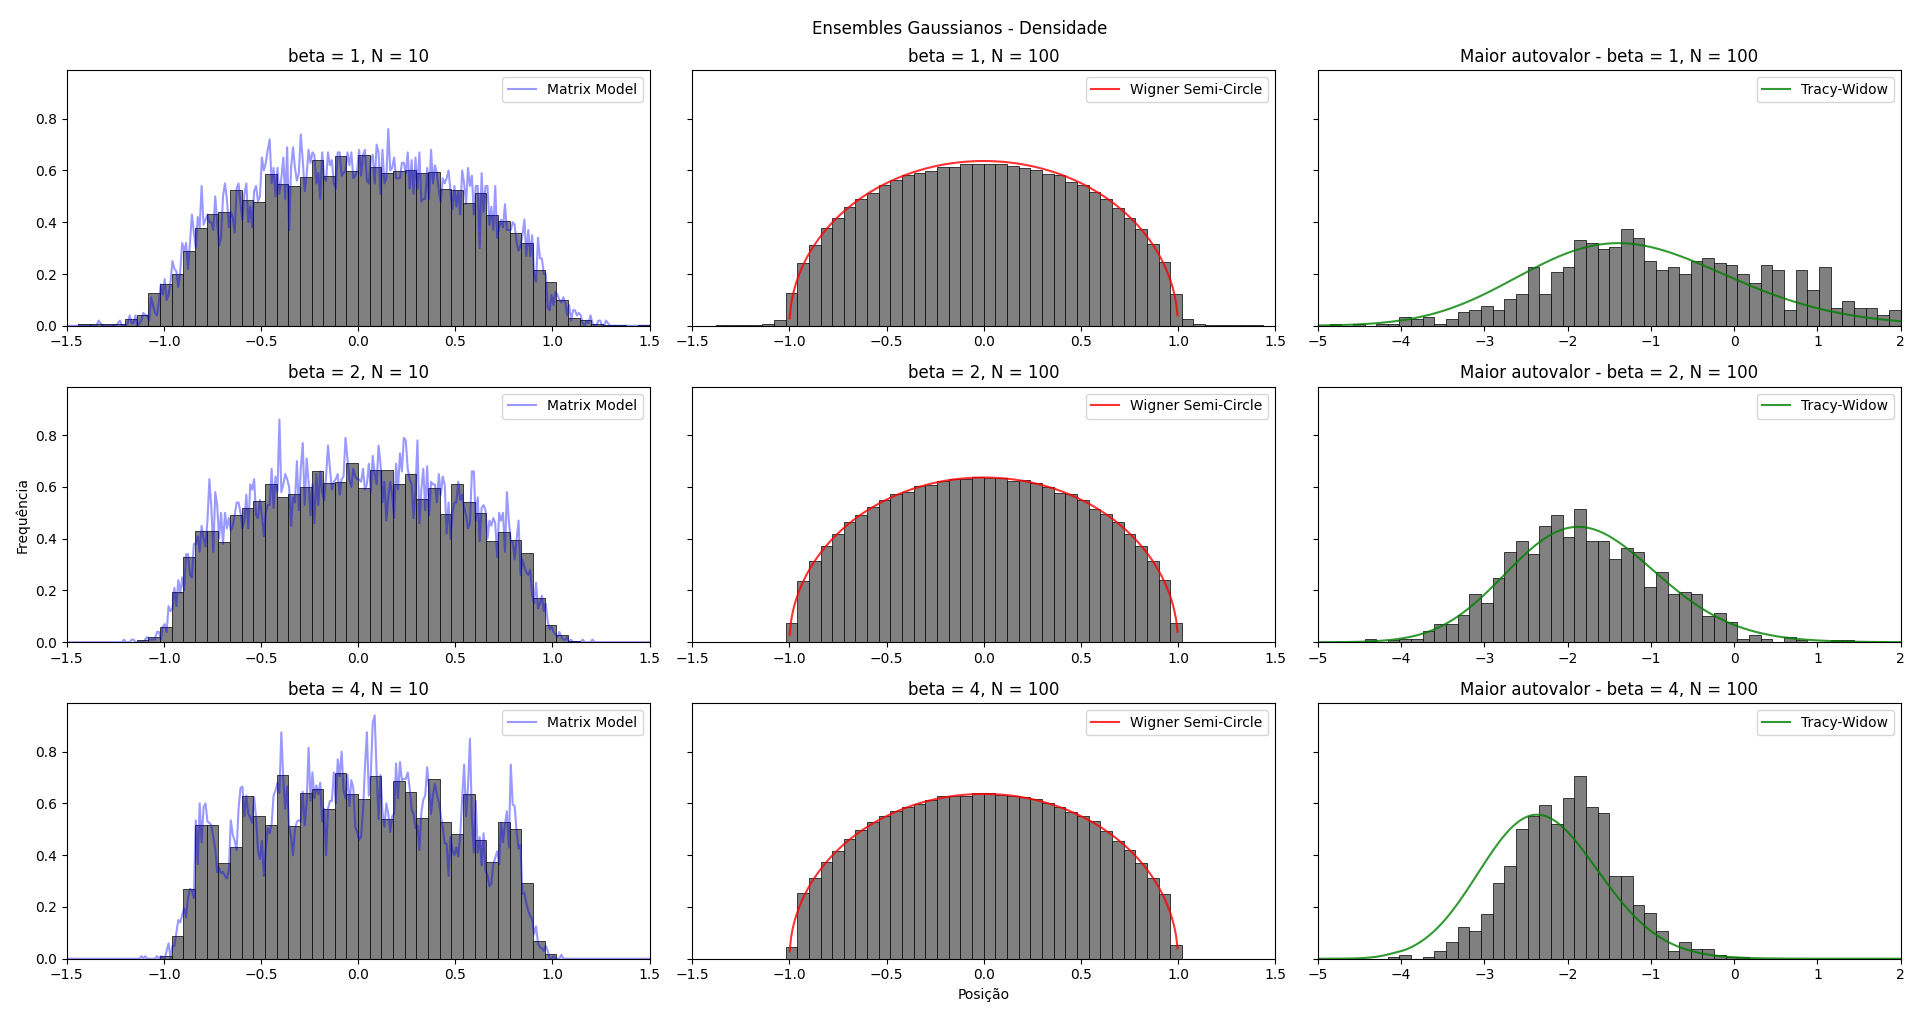
\includegraphics[width=\textwidth]{Assets/validationGaussianTracy.png}
	\caption{Densidade para ensembles gaussianos, \eqref{Equation: Parametros Gaussian}. Tomou-se $\Delta \tilde{t} = 0.1$ e $nsteps = 5\cdot10^6$ passos, registrando a cada $100$ iterações a partir de $nsteps/5$. À esquerda da figura, em azul, a densidade da amostragem de $4\cdot10^3$ matrizes do ensemble. No centro, o Semi-Círculo de Wigner, medida de equilíbrio. Na direita, apresenta-se a densidade de $\lambda_{max}$ normalizado e sua medida esperada.}
	\label{Figura: Gaussian}
\end{figure}

Podemos retomar também as descrições dos potenciais mônico, na Equação \eqref{Equação: Mônico}, e os dois regimes do potencial quártico, Caso \eqref{Equação: Quartico +} e Caso \eqref{Equação: Quartico -}. Respectivamente, estes modelos equivalem a tomar na simulação os parâmetros
\begin{equation}
	d = 1; \ \  n = 2; \ \ \V(x)= t |x|^{2m}; \ \ W(x) = g(x) = \log{|x|}; \ \ \beta_N = \beta N^2; \ \ \beta = 2.
	\label{Equation: Parametros Monico}
\end{equation}
\begin{equation}
	d = 1; \ \  n = 2; \ \ \V(x)=\frac{|x|^4}{4} + t \frac{|x|^2}{2}; \ \ W(x) = g(x) = \log{|x|}; \ \ \beta_N = \beta N^2; \ \ \beta = 2.
	\label{Equation: Parametros Quartico}
\end{equation}
O caso mônico se reduz ao gaussiano se $m=1$. Os resultados para ambos os potenciais estão explicitados na Figura \ref{Figura: Quartic Monic} para alguns parâmetros interessantes de $t$ e $m$.
\begin{figure}[ht!]
	\centering
	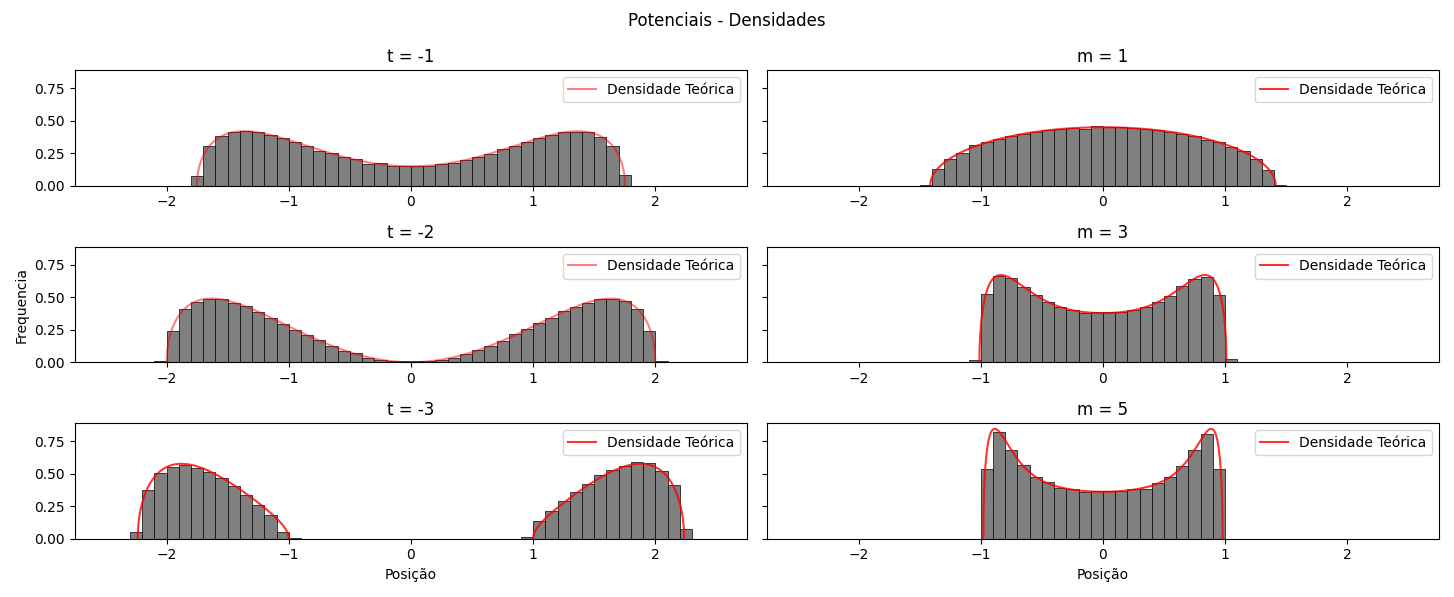
\includegraphics[width=\textwidth]{Assets/validationQuarticMonic-alt.png}
	\caption{Potencial Quártico \eqref{Equation: Parametros Quartico} e Mônico \eqref{Equation: Parametros Monico}, respectivamente à esquerda e direita. Tomou-se $\Delta \tilde{t} = 0.1$, $N=100$, e $nsteps = 5\cdot10^6$ passos. Registra-se a cada $1000$ iterações a partir de $nsteps/5$. No Quártico, simula-se $t=-1,-2,-3$. No Mônico fixa-se $t=1$ e simula-se $m=1,3,5$.}
	\label{Figura: Quartic Monic}
\end{figure}

Novamente as medidas experimentais parecem convergir para a medida teórica enunciada em todas as configurações testadas. Contudo, isso é discutido, com exceção do Mônico, por Chafa\"{i} e Ferré \cite{Chafa2018}. Em luz da situação recentemente explorada por Balogh \textit{et al.} \cite{balogh2016orthogonal} consideremos a Configuração \eqref{Equation: Complex} complexa. Para esta, representamos as medidas simuladas para alguns valores de interesse de $t, a$ na Figura \ref{Figura: Complex},
\begin{equation}
	d = 2; \  n = 2; \  \V(z)=|z|^{2a} - \Re{t z^a};  \ W(x) = g(x) = \log{|x|};  \ \beta_N = \beta N^2;  \ \beta = 2.
	\label{Equation: Complex}
\end{equation}

\begin{figure}[ht]
	\centering
	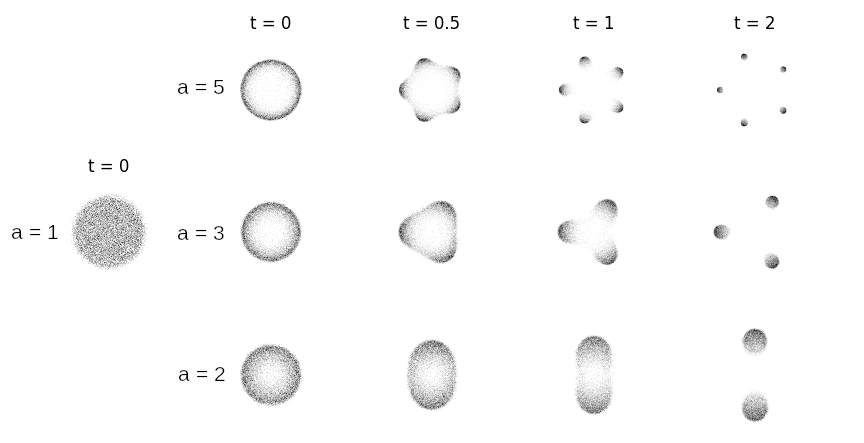
\includegraphics[width=\textwidth]{Assets/complexPotential.png}
	\caption{Medidas referentes à configuração \eqref{Equation: Complex}. Tomou-se $\Delta \tilde{t} = 0.5$ e $nsteps = 2\cdot10^6$ passos, registrando a cada $500$ iterações a partir de $nsteps/5$.}
	\label{Figura: Complex}
\end{figure}

É previsto para esse modelo uma transição de regime - uma separação da medida de equilíbrio - para $t_c \approx \sqrt{\frac{1}{a}}$, o que pode ser observado na Figura \ref{Figura: Complex} com algum detalhe. Outros fatores que corroboram o bom comportamento do modelo são que a medida é uniforme no disco quando $(a,t) = (1,0)$ e se concentra no bordo quando incrementa-se $a$, fatos também previstos. \cite{balogh2016orthogonal} Esse exemplo demonstra que é possível, sem muito esforço, replicar a medida, e principalmente o suporte, para potenciais mais complexos estudados em publicações recentes no tema e pode ser estendido para outros estudos, como para o potencial discutido por Bleher e Silva \cite{Silva}. 

No Capítulo \ref{Capitulo: Intro} apresentamos os ensembles gaussianos como os únicos ensembles invariantes de entradas independentes. Gerar matrizes de outros modelos invariantes dependeria de se saber construir matrizes de entradas não trivialmente correlacionadas. Por outro lado, se sabemos valer a decomposição espectral $\matriz{M} = \matriz{U} \matriz{\Lambda} \matriz{U}^{-1}$, resta que saibamos simular os autovalores para reconstruir as matrizes. Os autovetores podem ser amostrados uniformemente do espaço adequado nos ensembles invariantes. Agora, com a simulação de Gases de Coulomb, apresenta-se uma alternativa para tais distribuições de autovalores. Esse fato, por permitir a reconstrução destas matrizes, possibilita a exploração de múltiplas construções matemáticas que dependem de sua adequada amostragem.

%já que, se tratando de ensembles invariantes, podemos simular matriz $\matriz{U}$ de autovetores distribuídos uniformemente no espaço correspondente. Isso pois sabemos do teorema espectral que, para as matrizes tomadas, vale a decomposição $\matriz{M} = \matriz{U} \matriz{\Lambda} \matriz{U}^{-1}$. Para reconstruir um elemento do ensemble de interesse nos resta replicar a medida de autovalores da matriz $\matriz{\Lambda}$. Isso, de forma interessante, pode ser feito pela simulação descrita de Gases de Coulomb, que replica a medida dos autovalores dos ensemble.

%Outra possibilidade interessante da replicação numérica dessas medidas é que, miniminizada a energia livre $E_{N, V}$, podemos fazer estimativas para constantes da expansão para $\log(Z_{\beta_N})$ proposta em trabalhos recentes, como em \cite{Byun_2023}. Essas estimativas podem dar uma ideia geral do comportamento dessas constantes, de relevante significado físico, para sistemas de interesse.  


% -
% C3S3 - Outros Potenciais?
% - 
%\section{Além do usual}

Considere a seguinte configuração com potencial complexo e autovalores complexos ($\R^d = \R^2$)
\begin{equation}
	d = 2, \  n = 2, \  \V(z)=|z|^{2a} - \Re{(t z^a)},  \ W(x) = g(x) = \log{|x|},  \ \beta_N = \beta N^2,  \ \beta = 2.
	\label{Equation: Complex}
\end{equation}

\begin{figure}[ht]
	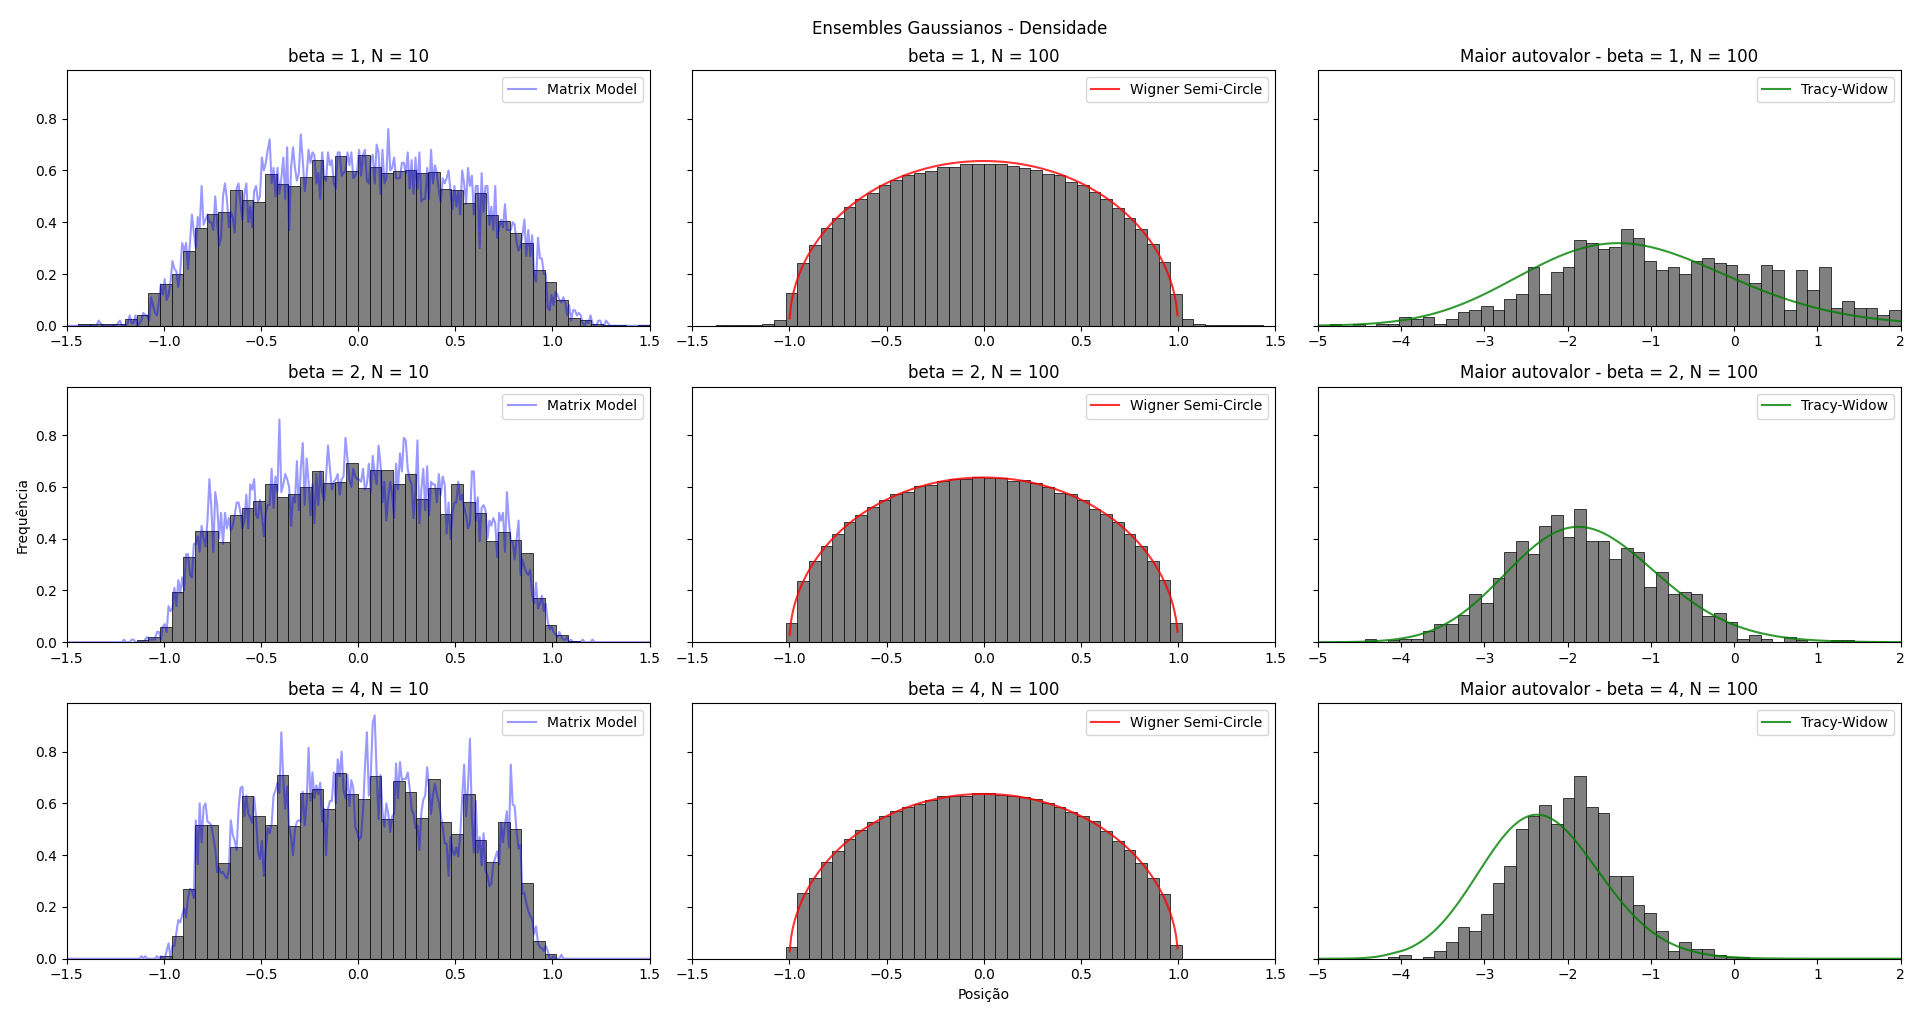
\includegraphics[width=\textwidth]{Assets/validationGaussianTracy.png}
	\caption{Medidas de equilíbrio para os ensembles gaussianos, equivalente à tomar \ref{Equation: Parametros Gaussian}. Para todos, vale a escolha de $\Delta t = 0.5$ e $nsteps = 2\cdot10^6$ passos, registrando a cada $1000$ iterações os microestados a partir da metade da simulação. Para as simulações à esquerda da figura se apresenta ainda a distribuição da amostragem de $10^6$ matrizes do tipo apropriado e a densidade resultante.}
	\label{Figura: Gaussian}
\end{figure}


% -
% C3S3 - Outros Potenciais?
% - 
%\section{Discussão}

É fácil ver para os casos \ref{Equation: Parametros Gaussian}, \ref{Equation: Parametros Monico}, \ref{Equation: Parametros Quartico} que as medidas explícita pela teoria são concordantes, como esperado, com a medida experimental obtida nas simulações. Contudo, isso é bem explorado e pode ser observado, com exceção do Mônico, em \cite{Chafa2018}. Foi discutido no Capítulo \ref{Capitulo: Intro} que os modelos gaussianos são os únicos em RMT com invariância por rotação e independência das entradas. Fica então a questão de como gerar matrizes de outros modelos se as entradas são correlacionadas. Sabemos do teorema espectral que, para as matrizes tomadas, vale a decomposição $\matriz{M} = \matriz{U} \matriz{D} \matriz{U}^{-1}$, já apresentada no Capítulo \ref{Capitulo: Intro}. Sabemos ainda que trataremos de ensembles invariantes, ou seja, a medida é a mesma para quaisquer $M, M'$ tais que $\matriz{M} = \matriz{U} \matriz{M'} \matriz{U}^{-1}$. Isso implica que podemos simular $\matriz{U}$ autovetores uniformemente do espaço correspondente. Para reconstruir uma elemento do ensemble de interesse nos resta replicar a medida de autovalores, $\matriz{D}$. Isso pode ser feito pela simulação descrita. Reconstruímos elementos dos ensembles a partir da simulação de sua medida com gases de Coulomb.


% ---
% Capítulo 4 - Conclusão
% ---

\chapter{Conclusão}
\label{Capitulo: Conclusão}

\lipsum[2-5]



% ----------------------------------------------------------
% ELEMENTOS PÓS-TEXTUAIS
% ----------------------------------------------------------
\postextual
% ----------------------------------------------------------

% -----------------------------------------------------------
% Referências bibliográficas
% ----------------------------------------------------------
\bibliography{USPSC-bib/USPSC-modelo-references}


% ----------------------------------------------------------
% Glossário
% ----------------------------------------------------------
%
% Consulte o manual da classe abntex2 para orientações sobre o glossário.
%
%\glossary

% ----------------------------------------------------------
% Apêndices
% ----------------------------------------------------------
%%% USPSC-Apendice.tex
% ---
% Inicia os apêndices
% ---

\begin{apendicesenv}
% Imprime uma página indicando o início dos apêndices
\partapendices
\chapter{Apêndice(s)}
Elemento opcional, que consiste em texto ou documento elaborado pelo autor, a fim de complementar sua argumentação, conforme a ABNT NBR 14724 \cite{nbr14724}.

Os apêndices devem ser identificados por letras maiúsculas consecutivas, seguidas de hífen e pelos respectivos títulos. Excepcionalmente, utilizam-se letras maiúsculas dobradas na identificação dos apêndices, quando esgotadas as 26 letras do alfabeto. A paginação deve ser contínua, dando seguimento ao texto principal. \cite{aguia2020}
% ----------------------------------------------------------
\chapter{Exemplo de tabela centralizada verticalmente e horizontalmente}
\index{tabelas}A \autoref{tab-centralizada} exemplifica como proceder para obter uma tabela centralizada verticalmente e horizontalmente.
% utilize \usepackage{array} no PREAMBULO (ver em USPSC-modelo.tex) obter uma tabela centralizada verticalmente e horizontalmente
\begin{table}[htb]
\ABNTEXfontereduzida
\caption[Exemplo de tabela centralizada verticalmente e horizontalmente]{Exemplo de tabela centralizada verticalmente e horizontalmente}
\label{tab-centralizada}

\begin{tabular}{ >{\centering\arraybackslash}m{6cm}  >{\centering\arraybackslash}m{6cm} }
\hline
 \centering \textbf{Coluna A} & \textbf{Coluna B}\\
\hline
  Coluna A, Linha 1 & Este é um texto bem maior para exemplificar como é centralizado verticalmente e horizontalmente na tabela. Segundo parágrafo para verificar como fica na tabela\\
  Quando o texto da coluna A, linha 2 é bem maior do que o das demais colunas  & Coluna B, linha 2\\
\hline
\end{tabular}
\begin{flushleft}
		Fonte: Elaborada pelos autores.\
\end{flushleft}
\end{table}

% ----------------------------------------------------------
\chapter{Exemplo de tabela com grade}
\index{tabelas}A \autoref{tab-grade} exemplifica a inclusão de traços estruturadores de conteúdo para melhor compreensão do conteúdo da tabela, em conformidade com as normas de apresentação tabular do IBGE.
% utilize \usepackage{array} no PREAMBULO (ver em USPSC-modelo.tex) obter uma tabela centralizada verticalmente e horizontalmente
\begin{table}[htb]
\ABNTEXfontereduzida
\caption[Exemplo de tabelas com grade]{Exemplo de tabelas com grade}
\label{tab-grade}
\begin{tabular}{ >{\centering\arraybackslash}m{8cm} | >{\centering\arraybackslash}m{6cm} }
\hline
 \centering \textbf{Coluna A} & \textbf{Coluna B}\\
\hline
  A1 & B1\\
\hline
  A2 & B2\\
\hline
  A3 & B3\\
\hline
  A4 & B4\\
\hline
\end{tabular}
\begin{flushleft}
		Fonte: Elaborada pelos autores.\
\end{flushleft}
\end{table}


\end{apendicesenv}
% ---

% ----------------------------------------------------------
% Anexos
% ----------------------------------------------------------
%%% USPSC-Anexos.tex
% ---
% Inicia os anexos
% ---
\begin{anexosenv}

% Imprime uma página indicando o início dos anexos
\partanexos

% ---
\chapter{Exemplo de anexo}
% ---
Elemento opcional, que consiste em um texto ou documento não elaborado pelo autor, que serve de fundamentação, comprovação e ilustração, conforme a ABNT NBR 14724. \cite{nbr14724}.

O \textbf{ANEXO B} exemplifica como incluir um anexo em pdf.

\chapter{Acentuação (modo texto - \LaTeX)}
\begin{figure}[H]
	\begin{center}
	\caption{\label{fig_anexob}Acentuação (modo texto - \LaTeX)}
	\includegraphics[scale=1.0]{USPSC-img/USPSC-AcentuacaoLaTeX.png} \\
	Fonte: \citeonline{comandos}
	\end{center}	
\end{figure}

\end{anexosenv}


%---------------------------------------------------------------------
% INDICE REMISSIVO
%--------------------------------------------------------------------
%%% USPSC-IndicexRemissivos.tex
% ---
% Inicia os Índices Remissivos
% ---
%---------------------------------------------------------------------
% INDICE REMISSIVO
%--------------------------------------------------------------------
\phantompart
\printindex
%---------------------------------------------------------------------


%---------------------------------------------------------------------

\end{document}
